\documentclass[a4paper,12pt,bibliography=totocnumbered, headings=small]{scrbook}
\usepackage[utf8]{inputenc} 
\usepackage[T1]{fontenc}
\usepackage[english]{babel} %Deutsche Zeichen- und Umbruchsetzung
\usepackage{amsmath, amssymb,amsfonts} %AMS-TeX-Pakete. Nötig für die Definition der Mathematik-Umgebung
\usepackage{bm}
\usepackage{graphicx} %Nötig, um Grafiken einbinden zu können
\usepackage[bookmarks,colorlinks=true]{hyperref} %Mittels hyperref lassen sich hyperlinks innerhalb des PDF-Dokumentes benutzen. Beispiel: Mausklick im Inhaltsverzeichnis auf ein Kapitel führt zum automatischen Sprung in dieses Kapitel
\usepackage{geometry}
\usepackage{float}
%Ein Paket, mit dem sich ohne Probleme mehrseitige PDF-Dokumente ohne \includegraphics-Rumgemache einbinden lassen. Befehl: \includepdf[pages=a-b]{PDFfile.pdf}. Einzelne Seiten, oder auch alle Seiten (Option pages=-) können angewählt werden
%Wenn keine Option angegeben wird, gilt pages=1!
\usepackage[final]{pdfpages}
\usepackage{framed, color} %Framed: Paket, mittels dessen ein Rahmen um einen Bereich definiert werden kann. Color: Lässt Farbdarstellung in Schrift, Hintergrund etc. zu
\usepackage{scrlayer-scrpage} %Header für die KOMA-script -Klasse
\usepackage{siunitx} %Ein schönes Paket, um Einheiten und physikalische Größen richtig zu setzen. Z.B.  \SI{2}{\kilo\gram\per\meter\squared}
\usepackage{graphicx}
\usepackage{placeins}
\usepackage{bbold}
\usepackage{subcaption} 
\usepackage[dvipsnames]{xcolor}
\usepackage[version=4]{mhchem}
\usepackage{tikz}
\usetikzlibrary{calc,arrows.meta,decorations.markings}
\usepackage[onehalfspacing]{setspace}

\usepackage{csquotes}
\usepackage[
  backend=biber,
  style=numeric,
  backref=true,
  backrefstyle=three
]{biblatex}

\addbibresource{lit.bib}


\usepackage{geometry}

\geometry{
   left=2.5cm,
   right=2.5cm,
   bottom=3.5cm,}
\usepackage{caption}
\captionsetup{format=plain, font=small,labelfont=bf}
%\captionsetup{justification=raggedright,singlelinecheck=false}
%siunitx-Konfiguration. Damit werden die richtigen Font-Einstellungen erkannt (also beispielsweise fett, kursiv etc.) und damit  ebenfalls die deutsche Zeichensetzung, insbesondere Trennungszeichen, benutzt werden. 
%Ebenso wird bei SIrange das "`to"' in "`bis"' umgewandelt, bei SIlist das "`and"' in "`und"'
\sisetup{
    detect-weight = true,
    detect-family = true,
    locale = US,              % or UK, depending on your thesis
    range-phrase = { to },
    list-final-separator = {, and },
    separate-uncertainty = true,
    per-mode = symbol-or-fraction
}
%\SI[per-mode = fraction]{1}{\meter\per\second} erzwingt auch im Fließtext die Bruchdarstellung.

%Hyperlinks-Setup
\hypersetup{
	colorlinks,
	linktocpage,
	citecolor=black,
	filecolor=black,
	linkcolor=black,
	urlcolor=black
}

\numberwithin{equation}{chapter} % Die Nummerierung von Gleichungen bekommt die jeweilige Section-Nummer als Präfix

\setlength{\parindent}{0 mm} %Einrücktiefe von neuen Absätzen
\setlength{\parskip}{2 mm} %Abstand von Absätzen



\pagestyle{scrheadings}%Kopf und Fußzeilen
\ohead{\empty} %Header oben links auf linker Seite (ungerade Seitenzahl) und oben rechts auf rechter Seite (gerade Seitenzahl), beinhaltet gruppennummer und Versuchskürzel. Im Fall eine einseitigen Dokuments: Header oben rechts
\ihead{\empty} %Header oben rechts auf linker Seite und oben links auf rechter Seite. Beinhaltet die Namen der Verfasser. Im Fall eine einseitigen Dokuments: Header oben links!
\ofoot{\thepage} %Footer unten links auf linker und unten rechts auf rechter Seite, enthält die jeweilige Seitenzahl. Im Fall eines einseitigen Elements: Footer unten rechts!
\cfoot{\empty} %Mittig unten im Footer soll nichts eingetragen werden 
\ifoot{\empty} %Footer unten rechts auf linker und unten links auf rechter Seite. Hier ebenfalls leer.


%%%%%%%%%%%%%%%%%%%%%%%%%%%%%%%%%%%%%%%%%%%%%%%%%%%%%%%%%%%%%%%%%%%%%%%%%%%%%%%%%%%%%%%%%%%%%%%%%%%%%%%%%%%%%%%%%%%%%%%%%%%%%%%%%%%%%%%%%%%%

% Hier können die individuellen Anpassungen vorgenommen werden, die sich auf das Titelblatt und die Kopfzeilen auswirken.


\newcommand{\PROTOKOLLDATUM}{\today}



\newcommand{\VerfasserZWEI}{Tim Heinkele}
\newcommand{\MatNoZWEI}{3693236}
\newcommand{\bra}[1]{\langle #1 \rvert}
\newcommand{\ket}[1]{\lvert #1 \rangle}
\newcommand{\braket}[2]{\langle #1 \mid #2 \rangle}
\newcommand{\doubleunderline}[1]{\underline{\underline{#1}}}



\newlength{\spinlen}
\setlength{\spinlen}{6mm}
\def\halflen{3mm}
\tikzset{
  mid arrow/.style={
    postaction={
      decorate,
      decoration={
        markings,
        mark=at position .6 with {\arrow{Stealth[scale=1.3]}}
      }
    }
  }
}


\tikzset{
  spin/.style={->, ultra thick, >=Stealth}
}
\newcommand{\centerspin}[3][]{%
  \begin{scope}[shift={#2}, rotate=#3]
    \draw[spin,#1] (-\spinhalf,0) -- (\spinhalf,0);
  \end{scope}%
}

\newcommand{\BETREUERIN}{Dr. Jessica  Almeida}
\newcommand{\BETREUER}{Prof. Dr. Mathias S. Scheurer}
\definecolor{pastelgreen}{HTML}{2E8B57}
\definecolor{pastelblue}{HTML}{2F84FB}
\definecolor{pastelred}{HTML}{FC6061}
\definecolor{brown}{HTML}{964D1E}
\definecolor{purple}{HTML}{4F1A73}



\begin{document}

\thispagestyle{empty}


\begin{titlepage}

\begin{center}
\vspace*{17mm}

\includegraphics[width=0.6\linewidth]{Pictures/unistuttgart_logo_englisch_cmyk-01.png}


\vspace{1cm}
\large{Institute for Theoretical Physics III} \\
\vspace{2cm}
\normalsize{Bachelor's thesis} \\
\vspace{1cm}
\Huge{Altermagnetism on the Kagome lattice}\\% \Huge \huge \Large \normalsize \Small usw. bestimmt die Schriftgröße.
\vspace{1cm}% Abstand
\normalsize{Tim Heinkele} \\
\vspace{5mm} 
\normalsize{\today}\\
\vspace{6cm}
\normalsize{Supervised by}\\
\normalsize{\BETREUER{} and \BETREUERIN{}}
\end{center}




\end{titlepage}


\newpage
\thispagestyle{empty}
~
\newpage

\chapter*{Declaration}
I hereby declare, that I have written the Bachelor's thesis by myself at the Institute of Theoretical Physics under supervision of Dr. Jessica Almeida and that all sources are signposted and cited. I used OpenAI's ChatGPT to assist in developing and modifying the underlying code of numerical computations. The content and conclusions are my own work. The Bachelor's thesis has not been submitted elsewhere. Lastly, I insure that the printed copy is identical to the electronic version.
\newpage

\thispagestyle{empty}

\chapter*{Abstract}

When a material permits spin-split bands while having compensated magnetic order, we speak of altermagnets.
In this thesis, altermagnets are being analyzed under the influence of different magnetic textures, breathing distortions of the lattice and Rashba-spin-orbit coupling (Rashba-SOC).  \\

For this, we introduce a two-dimensional tight binding model for the magnetic order of the T1 and T2 phase of \ce{Mn3Pt}, of \ce{Mn3Ge} and \ce{Mn3Sn}. An unitary transformation of the tight-binding Hamiltonian is used to achieve cell-periodic states. For the computation of the Berry curvature, we use the Fukui-Hatsugai-Suzuki method and additionally a composite representation for degenerate bands.
Subsequently, the band structure, Fermi-surface spin texture, Berry curvature and Chern number are computed for the different magnetic textures.\\
Here, we develop a theory for the symmetries holding on the magnetic textures and adapt them on the computations, confirming our theory. \\

In \ce{Mn3Ge} and \ce{Mn3Sn} we find a symmetry, imposing $C_{3z}$-symmetric behavior. The numerical computations show behavior, imposed by $\mathcal{TM}$ planes, for the T1 phase of \ce{Mn3Pt} and \ce{Mn3Ge}, which is assumed to hold in the presence of SOC.
In the nonbreathing limit without SOC, symmetries force the Berry curvature to vanish.
The T1 and T2 phase of \ce{Mn3Pt}, as well \ce{Mn3Ge} and \ce{Mn3Sn}, give equivalent results in the absence of SOC because their magnetic order differ by a global spin rotation.\\
Breathing distortions in the absence of SOC allow an odd Berry curvature in momentum, imposing a vanishing Chern number.\\
Using the received symmetries, we show that \ce{Mn3Pt} cannot exhibit an in-plane net magnetization, whereas \ce{Mn3Ge} \ce{Mn3Sn} can exhibit one along distinct directions in the presence of SOC. The examined materials remain spin-split in the absence of SOC, identifying them as strong altermagnets. Due to the in-plane net magnetization, \ce{Mn3Ge} and \ce{Mn3Sn} are identified as M-type altermagnets and T1 and T2 \ce{Mn3Pt} as S-type altermagnets.\\

% In general we find the symmetries $[E||C_{2z}]$, holding in the nonbreathing limit for  and $\Theta_s[C_{2z}||E]$ holding in the absence of SOC.

% \ce{Mn3Pt} is confirmed of S-type, where the T1 phase can exhibit an out-of plane net magnetization and T2 has a compensated net magnetization, as also stated in Ref.~\cite{Quelle3}.
% For \ce{Mn3Ge} and \ce{Mn3Sn} we find the $[C_{3z}||C_{3z}^{-1}]$-symmetry, enabling an in-plane net-magnetization along the $y$-axis, or along the $x$-axis, respectively, due to the additional $\mathcal{TM}$ and $\mathcal{M}$ planes.
% With the numerical computations, we assume the $\mathcal{TM}$ planes to be conserved in the presence of SOC.\\
% 

\newpage
\thispagestyle{empty}

\chapter*{Zusammenfassung}
\newpage
\thispagestyle{empty}

 
\tableofcontents
\thispagestyle{empty}


\newpage
\thispagestyle{empty}
~
\newpage

\clearpage 
\setcounter{page}{1}

\chapter{Introduction}

\label{chapter: Introduction}
Altermagnetism has become an emerging topic in the field of spintronics and magnetism. Altermagnets combine properties of ferro- and antiferromagnets: They have spin-split bands, while their magnetic order is fully compensated. Because of their vanishing or small net magnetization, they represent promising candidates for spintronics due to their weak magnetic stray fields and therefore are robust against external magnetic fields.\\
Despite their compensated magnetic order, they can exhibit properties that are common in ferromagnets. One example for this is the anomalous Hall effect (AHE), which was studied for different compounds in Refs.~\cite{PhysRevB.111.184407, Quelle2, MnPtSOC}. \\
Altermagnetism has also attracted interest in the context of superconductivity \cite{PhysRevB.108.224421},  where the superconducting diode effect (SDE)  was studied in altermagnets \cite{cv8s-tk4c, Quelle3}. \\

Originally, altermagnetism was introduced for collinear systems \cite{PhysRevX.12.040501} and was later extended to noncollinear magnetic systems \cite{Cheong2024, Cheong2025}. Due to their geometry, kagome lattices support $120^\circ$ magnetic order and therefore supply a great platform to achieve noncollinear altermagnets. Depending on their magnetic order and the corresponding symmetries, they can realize different types of altermagnetism, which are classified in Ref. \cite{Cheong2025}. A few examples of noncollinear altermagnets include \ce{Mn3Pt}, \ce{Mn3Ge} and \ce{Mn3Sn}.

For the study of the compounds, different theoretical methods can be used, including first-principles calculations \cite{Quelle2, Yang_2017}, Monte Carlo simulations \cite{9d8q-cjk7} and tight-binding models \cite{PhysRevB.99.165141}.
In this thesis, a tight-binding model is used to provide a simple description of the electronic structure, to simplify symmetry analysis, and to allow the effects of spin-orbit coupling and different magnetic orders to be studied separately. \\

In this thesis, we aim to describe the electronic-structure properties, namely the electronic band structure, Fermi-surface spin texture and Berry curvature, for the magnetic textures of the T1 and T2 phases of \ce{Mn3Pt} and of \ce{Mn3Ge} and \ce{Mn3Sn}, on regular and breathing kagome lattices with and without Rashba-SOC. The model for \ce{Mn3Pt} follows Ref. \cite{Quelle3}, which serves as a guide in this thesis. 
In Chapter \ref{chapter:Theory}, the tight-binding model and the Berry curvature are introduced, together with the different types of altermagnetism and their relevant symmetries.
Then, in Chapter \ref{chapter:Results}, the model introduced above is applied to the different magnetic textures, the relevant symmetries are identified and
their predictions are compared with the numerical results.
Finally, Chapter \ref{chapter: conclusion} summarizes the main findings and gives an outlook on further extensions.\\








\chapter{Basics}
\label{chapter:Theory}

In order to theoretically analyze a crystal structure for its different properties, a model has to be selected. \\
In condensed-matter physics, a tight-binding model has become a standard in recent decades. The Haldane model \cite{Haldane_1988} served as a stepping stone for subsequent models such as the Kane-Mele model \cite{Kane_2005}. \\
In this chapter, the tight-binding model for a kagome lattice, altermagnetism and important symmetries are introduced. 

\section{Tight-binding model}
\label{section: tightbinding}
% In this work, a electron tight-binding Hamiltonian with pure Rashba-Spin-orbit coupling (Rashba-SOC) and a magnetic texture is being used to compute the electronic spectra and further properties, where the electrons hop between different $\ce{Mn}$ sites with varying magnetic moments, defining the magnetic texture. 
With an electronic tight-binding model, the motion of electrons in a crystal structure can be described. For the compounds considered here, the relevant crystallographic plane forms a kagome lattice, shown in Fig.~\ref{fig: kagome_model_definitions}.

The total Hamiltonian $H = H_0+ H_\text{R}+ H_\text{M}$, describing the system, consists of three parts, where $H_0$ describes the nearest-neighbor hopping, $H_\text{R}$ the pure Rashba spin-orbit coupling (hereafter abbreviated as SOC) and $H_\text{M}$ the local magnetic exchange term. \\
The hopping Hamiltonian is defined as
\begin{align}
H_0 = -\sum_{\mathbf R} \Bigg\{& t' \sum_{i=1}^{3} \mathbf{c}_{\mathbf R,\beta_i}^{\dagger} \mathbf{c}_{\mathbf R,\alpha_i} 
+t \sum_{i=1}^{3} \mathbf{c}_{\mathbf R-\mathbf a_i,\beta_i}^{\dagger} \mathbf{c}_{\mathbf R,\alpha_i} \Bigg\} +\mathrm{H.c.},
\label{eq: 1_hamiltonian_hopping}
\end{align}
where the creation and annihilation operators, $\mathbf{c}_{\mathbf{R},\alpha_i}^\dagger$ and $\mathbf{c}_{\mathbf{R},\alpha_i}$, are used with $\mathbf{c}_{\mathbf R,\alpha}^{\dagger}
  =
  \left(
  c_{\mathbf R,\alpha\uparrow}^{\dagger},
  c_{\mathbf R,\alpha\downarrow}^{\dagger}
  \right)$ or 
  $\mathbf{c}_{\mathbf R,\alpha}
  =
  \begin{pmatrix}
  c_{\mathbf R,\alpha\uparrow}\\
  c_{\mathbf R,\alpha\downarrow}
  \end{pmatrix}$
 respectively with the sublattices 
$$
(\alpha_i,\beta_i) = \begin{cases}
(A,B), & i=1,\\
(B,C), & i=2,\\
(C,A), & i=3.
\end{cases}
$$
Here, the hopping amplitudes are defined as $t_i=t$ for the downward and $t'_i=t'$ for the upward facing triangles with $i\in\{1,2,3\}$, depicted in Fig. \ref{fig: kagome_model_definitions}. Note that the model can be adjusted by also adding distortions in the equilateral triangles, by choosing $t_i \neq t_j$ for $i\neq j$. In our case, we choose $t_i = t_j$. The case for $t=t'$ and $\lambda = \lambda'$ is called nonbreathing limit, describing a kagome lattice with equal-sized upward- and downward-facing triangles.
 with the annihilation spinor defined as the column vector
 
\begin{figure}[tbhp]
    \centering
    \centering
    \begin{tikzpicture}[scale=1.8]
    
    \draw[thick] ({1/2}, {sqrt(3)/2}) -- ({1}, {sqrt(3)}) -- ({3/2}, {sqrt(3)/2}) -- ({1/2}, {sqrt(3)/2});
    \draw[thick] ({3/2}, {sqrt(3)/2}) -- ({5/2}, {sqrt(3)/2}) -- ({2}, {0}) -- ({3/2}, {sqrt(3)/2});
    \draw[thick] ({2}, {0}) -- ({5/2}, {-sqrt(3)/2}) -- ({3/2}, {-sqrt(3)/2}) -- ({2}, {0});
    \draw[thick] ({1/2}, {-sqrt(3)/2}) -- ({1}, {-sqrt(3)}) -- ({3/2}, {-sqrt(3)/2}) -- ({1/2}, {-sqrt(3)/2});
    \draw[thick] ({-1/2}, {sqrt(3)/2}) -- ({-1}, {sqrt(3)}) -- ({-3/2}, {sqrt(3)/2}) -- ({-1/2}, {sqrt(3)/2});
    \draw[thick] ({-3/2}, {sqrt(3)/2}) -- ({-5/2}, {sqrt(3)/2}) -- ({-2}, {0}) -- ({-3/2}, {sqrt(3)/2});
    \draw[thick] ({-2}, {0}) -- ({-5/2}, {-sqrt(3)/2}) -- ({-3/2}, {-sqrt(3)/2}) -- ({-2}, {0});
    \draw[thick] ({-1/2}, {-sqrt(3)/2}) -- ({-1}, {-sqrt(3)}) -- ({-3/2}, {-sqrt(3)/2}) -- ({-1/2}, {-sqrt(3)/2});
    
    \draw[thick] ({0}, {0}) -- ({1/2}, {sqrt(3)/2}) -- ({-1/2}, {sqrt(3)/2}) -- ({0}, {0});
    \draw[thick] ({0}, {0}) -- ({1/2}, {-sqrt(3)/2}) -- ({-1/2}, {-sqrt(3)/2}) -- ({0}, {0});
    
    \draw[mid arrow, pastelred, very thick, dashed] ({1/2}, {sqrt(3)/2}) -- ({-1/2}, {sqrt(3)/2}) node[midway, above right,  pastelred] {$t_2$};
    \draw[mid arrow, pastelred, very thick, dashed] ({-1/2}, {sqrt(3)/2}) -- ({0}, {0}) node[midway,left, xshift=-5pt,pastelred] {$t_3$};
    \draw[mid arrow, pastelred, very thick, dashed] ({0}, {0}) -- ({1/2}, {sqrt(3)/2}) node[midway,right, xshift=5pt, pastelred] {$t_1$};
    
    \draw[mid arrow, pastelblue, very thick, dashed] ({-1/2}, {-sqrt(3)/2}) -- ({1/2}, {-sqrt(3)/2}) node[midway, below, yshift=-5pt, pastelblue] {$t'_2$};
    \draw[mid arrow, pastelblue, very thick, dashed] ({0}, {0}) -- ({-1/2}, {-sqrt(3)/2}) node[midway, left, xshift=-5pt, pastelblue] {$t'_1$};
    \draw[mid arrow, pastelblue, very thick, dashed] ({1/2}, {-sqrt(3)/2}) -- ({0}, {0}) node[midway,right, xshift=5pt, pastelblue] {$t'_3$};
    \draw[spin, black, thick] (1,{0}) -- (3/2,0) node[midway, below right] {$\mathbf{\hat{x}}$};
    \draw[spin, black, thick] (1,{0}) -- (1,{1/2}) node[midway, above right] {$\mathbf{\hat{y}}$};
    \filldraw[color=black, fill= white, thick]({1,{0}}) circle (1.5pt);
    \filldraw[color=black, fill= black, very thick]({1,{0}}) circle (0.3pt) node[below, xshift=-2pt] {$\mathbf{\hat{z}}$};
    \draw[spin, pastelgreen] (-1,{0}) -- (1,{0}) node[midway, below right, xshift=6pt] {$\mathbf{a}_2$};
    \draw[spin, pastelgreen] ({-1},{0}) -- ({-2}, {sqrt(3)}) node[midway, above right, yshift=9pt, xshift=-9pt] {$\mathbf{a}_3$};
    \draw[spin, pastelgreen] ({-1}, {0}) -- ({-2},{-sqrt(3)}) node[midway, below left, yshift=-1pt, xshift=-5pt] {$\mathbf{a}_1$};
    
    \filldraw[color=black, fill= black, very thick]({1}, {sqrt(3)}) circle (1.2pt);
    \filldraw[color=black, fill= black, very thick]({1}, {-sqrt(3)}) circle (1.2pt);
    \filldraw[color=black, fill= black, very thick]({-1}, {-sqrt(3)}) circle (1.2pt);
    \filldraw[color=black, fill= black, very thick]({-1}, {sqrt(3)}) circle (1.2pt) node[right, xshift=3pt] {A};
    \filldraw[color=black, fill= black, very thick]({2}, {0}) circle (1.2pt);
    \filldraw[color=black, fill= black, very thick]({-2}, {0}) circle (1.2pt);
    \filldraw[color=black, fill= black, very thick]({0}, {0}) circle (1.2pt);
    
    \filldraw[color=black, fill= black!40, very thick]({-3/2}, {sqrt(3)/2}) circle (1.2pt) node[below right, xshift=3pt] {B};
    \filldraw[color=black, fill= black!40, very thick]({1/2}, {sqrt(3)/2}) circle (1.2pt);
    \filldraw[color=black, fill= black!40, very thick]({5/2}, {sqrt(3)/2}) circle (1.2pt);
    \filldraw[color=black, fill= black!40, very thick](-{5/2}, {-sqrt(3)/2}) circle (1.2pt);
    \filldraw[color=black, fill= black!40, very thick]({3/2}, {-sqrt(3)/2}) circle (1.2pt);
    \filldraw[color=black, fill= black!40, very thick]({-1/2}, {-sqrt(3)/2}) circle (1.2pt);
    
    \filldraw[color=black, fill= white, very thick]({3/2}, {sqrt(3)/2}) circle (1.2pt);
    \filldraw[color=black, fill= white, very thick](-{1/2}, {sqrt(3)/2}) circle (1.2pt)  node[above right] {C};
    \filldraw[color=black, fill= white, very thick](-{5/2}, {sqrt(3)/2}) circle (1.2pt);
    \filldraw[color=black, fill= white, very thick]({5/2}, {-sqrt(3)/2}) circle (1.2pt);
    \filldraw[color=black, fill= white, very thick]({-3/2}, {-sqrt(3)/2}) circle (1.2pt);
    \filldraw[color=black, fill= white, very thick]({1/2}, {-sqrt(3)/2}) circle (1.2pt);

    
    \def\spinlen{0.2}
    \def\spinhalf{0.2}

    % useful constants
    \pgfmathsetmacro{\rt}{sqrt(3)}
    \pgfmathsetmacro{\rtHalf}{sqrt(3)/2}
    \pgfmathsetmacro{\rtQuarter}{sqrt(3)/4}
    \pgfmathsetmacro{\threeRtQuarter}{3*sqrt(3)/4}

    \draw[thick]
      (5,0) -- (5.5,\rtHalf) -- (4.5,\rtHalf) -- (5,0);

    \draw[thick]
      (5.5,-\rtHalf) -- (5,0) -- (4.5,-\rtHalf) -- (5.5,-\rtHalf);

    \centerspin[pastelblue, dashed]{(5,-\rtHalf)}{90}
    \centerspin[pastelblue, dashed]{(4.75,-\rtQuarter)}{330}
    \centerspin[pastelblue, dashed]{(5.25,-\rtQuarter)}{210}

    \centerspin[pastelred]{(5,\rtHalf)}{90}
    \centerspin[pastelred]{(4.75,\rtQuarter)}{210}
    \centerspin[pastelred]{(5.25,\rtQuarter)}{330}

    % \node[text=pastelblue, draw=none] at (1.1, 0.5) {$d_1$};
    % \node[text=pastelblue, draw=none] at (0, 0.5) {$d_1$};
    % \node[text=pastelblue, draw=none] at (0.625, -0.25) {$d_1$};

    \node[text=black, draw=none] at (5.5, {(0.5+\rt)/4}) {$\mathbf{d}_1$};
    \node[text=black, draw=none] at (5.2, {(0.5+\rt)/2}) {$\mathbf{d}_3$};
    \node[text=black, draw=none] at (4.5, {(0.5+\rt)/4}) {$\mathbf{d}_2$};
    \filldraw[color=black, fill= black, very thick]({5}, {0}) circle (1.2pt);
    \filldraw[color=black, fill= black!40, very thick]({4.5}, {-\rtHalf}) circle (1.2pt);    
    \filldraw[color=black, fill= black!40, very thick]({5.5}, {\rtHalf}) circle (1.2pt);
    \filldraw[color=black, fill= white, very thick]({5.5}, {-\rtHalf}) circle (1.2pt);         
    \filldraw[color=black, fill= white, very thick]({4.5}, {\rtHalf}) circle (1.2pt);    
    \node[text=black, draw=none] at (-3, {(0.1+\rt)}) {$\mathbf{(a)}$};
    \node[text=black, draw=none] at (4, {(0.1+\rt)}) {$\mathbf{(b)}$};
    \end{tikzpicture}
    \caption{kagome lattice showing the definitions of (a) the hopping amplitudes $t_i$ and the cell-connection vectors $\mathbf{a}_i$ and (b) the SOC bonding orientation vectors $\mathbf{d}_i$.}
    \label{fig: kagome_model_definitions}
\end{figure}
The Pauli matrices later used are defined as
\begin{align}
    \bm{\hat{\sigma}} = \begin{pmatrix}
        \hat{\sigma}_x\\ \hat{\sigma}_y\\ \hat{\sigma}_z
    \end{pmatrix} \qquad 
    \hat{\sigma}_x = \begin{pmatrix}0 & 1 \\ 1& 0
    \end{pmatrix}, \quad 
    \hat{\sigma}_y = \begin{pmatrix}0 & -i \\ i& 0 \end{pmatrix},\quad \text{and} \quad \hat{\sigma}_z = \begin{pmatrix}1 & 0 \\ 0& -1 \end{pmatrix}.
    \label{eq: pauli matrices}
\end{align}  

For the pure Rashba-SOC term 
% \begin{align}
%     H_\text{R} =  i \sum_{\mathbf{R}}   &\left(\lambda' \big[\mathbf{c}_{\mathbf{R}B}^\dagger (\mathbf{d_1}\cdot \bm{\sigma})\mathbf{c}_{\mathbf{R}A} + \mathbf{c}_{\mathbf{R}C}^\dagger  (\mathbf{d_2}\cdot \bm{\sigma}) \mathbf{c}_{\mathbf{R}B} + \mathbf{c}_{\mathbf{R}A}^\dagger  (\mathbf{d_3}\cdot \bm{\sigma})\mathbf{c}_{\mathbf{R}C} \big] \right.\\ 
%     &+ \left. \lambda \big[ c_{(\mathbf{R-a_1})B}^\dagger  (\mathbf{d_1}\cdot \bm{\sigma}) \mathbf{c}_{\mathbf{R}A} 
%         + c_{(\mathbf{R-a_2})C}^\dagger  (\mathbf{d_2}\cdot \bm{\sigma})\mathbf{c}_{\mathbf{R}B} 
%         + c_{(\mathbf{R-a_3})A}^\dagger  (\mathbf{d_3}\cdot \bm{\sigma})\mathbf{c}_{\mathbf{R}C} \big] \right)+ \text{H.c} .
%         \label{eq: Rashba Hamiltonian soc}
% \end{align}

\begin{align}
H_{\mathrm R}
=
i\sum_{\mathbf R}
\Bigg\{
&
\lambda'
\sum_{i=1}^{3}
\mathbf{c}_{\mathbf R,\beta_i}^{\dagger}
(\mathbf d_i\!\cdot\!\hat{\bm{\sigma}})
\mathbf{c}_{\mathbf R,\alpha_i}
+
\lambda
\sum_{i=1}^{3}
\mathbf{c}_{\mathbf R-\mathbf a_i,\beta_i}^{\dagger}
(\mathbf d_i\!\cdot\!\hat{\bm{\sigma}})
\mathbf{c}_{\mathbf R,\alpha_i}
\Bigg\}
+\mathrm{H.c.},
\label{eq:Rashba_Hamiltonian_soc}
\end{align}
the bond-orientation vectors $\mathbf{d}_1=(\sqrt{3}/2,\,-1/2,\, 0)^{\mathrm T}$, $\mathbf{d}_2=(0,\,1,\, 0)^{\mathrm T}$ and 
$\mathbf{d}_3=(-\sqrt{3}/2,\,-1/2,\, 0)^{\mathrm T}$ and cell-connection vectors, defined as $\mathbf{d}_i = \mathbf{\hat{e}}_z\times\mathbf{a_i}$ with $\mathbf{a}_1  = (-1/2,\,-\sqrt{3}/2,\, 0)^{\mathrm T}$, $\mathbf{a}_2 = (1,\,0)^{\mathrm T}$ and $\mathbf{a}_3 = (-1/2,\,\sqrt{3}/2,\, 0)^{\mathrm T}$ are used, which are depicted in Fig. \ref{fig: kagome_model_definitions} with $\bm{\hat{\sigma}}$ defined in Eq. \eqref{eq: pauli matrices}.  The dashed bonding orientation vectors in \ref{fig: kagome_model_definitions} (b) resemble the Hermitian conjugate and therefore the switched sign of the imaginary unit. 
Rashba-SOC requires structural inversion asymmetry normal to the $xy$-plane, as stated in Ref. \cite{Manchon2015}, and therefore can, for example be induced by applying an out of plane electrical field or by stacking polar planes as achieved by f.e. coupling the system to a superconducter, treating both sides $z$ and $-z$ differently, as executed in reference \cite{Quelle3}. This makes the two sides of the kagome plane distinguishable and therefore breaks the in-plane mirror symmetry. 
Note, that we might also expect an intrinsic SOC in the examined kagome materials. To include intrinsic SOC, the model can be adjusted by adding a similar term as the Rashba-SOC term \eqref{eq:Rashba_Hamiltonian_soc}, but with $\mathbf{d}_i = \mathbf{e}_z$ as used in \cite{PhysRevB.99.165141}, where the tight-binding Hamiltonian is similarly defined, which will eventually split the spin-split bands further. Furtheron, only pure Rashba-SOC is used. 
\\
In detail, the Rashba-SOC Hamiltonian is created by modifying the general Hamiltonian
\begin{align}
    H_\text{R} = (\alpha_R/\hbar) \left(\mathbf{\hat{e}}_z\times \mathbf{p}\right) \cdot \bm{\sigma}
    \label{eq: Rashba_Hamiltonian_standard}
\end{align}
as in Ref. \cite{Bychkov1984OscillatoryEA}.
By using a discretization of the continous Hamiltonian and switching into quantum mechanics, analogously as in \cite{PhysRevB.94.184402}, the original Hamiltonian \eqref{eq:Rashba_Hamiltonian_soc} is achieved. Here, we use $\mathbf{p}\to \hat{\mathbf{p}} = -i\hbar\bm{\nabla}$ and obtain 
\begin{align}
    H_\text{R} = -i\alpha_\text{R}(\mathbf{\hat{e}}_z \times \bm{\nabla})\cdot \bm{\hat{\sigma}}.
\end{align}. Lastly, defining a finite difference $\bm{{\delta}}_{ij}$ along directed bonds, produces 
\begin{align}
    H_\text{R} = i \sum_{\langle ij\rangle} \lambda_{ij} \mathbf{c}_i^\dagger [(\bm{\hat{e}}_{z}\times \bm{{\delta}}_{ij}) \cdot \bm{\hat{\sigma}}] \mathbf{c}_j + \text{H.c.}.
\end{align}
Hence, the imaginary unit originates from the momentum operator $-i\hbar\bm{\nabla}$.  
Furtheron, the direction simplifies to the direction of the bonding orientation vectors $\mathbf{d}_i = \mathbf{\hat{e}}_z \times \bm{\delta}_{ij}$ as defined in Fig. \ref{fig: kagome_model_definitions}. 

The magnetic texture Hamiltonian $H_\text{M}$ is defined as
\begin{align}
    H_\text{M} = -m_0 \sum_\mathbf{R} \sum_\alpha \mathbf{c}_{\mathbf{R},\alpha}^\dagger \left( \mathbf{m}_\alpha\cdot \mathbf{\hat{\sigma}}\right) \mathbf{c}_{\mathbf{R},\alpha},
    \label{eq: hamiltonian magnetic texture}
\end{align}
which directed local magnetic texture $\mathbf{m}_\alpha$, with $|\mathbf{m}_\alpha=1|$ acts on each sublattice $\alpha$ with the strength $m_0\geq 0$. It can easily be seen, that this term is also hermitian. The sign is defined, that anti-aligning spins with the magnetic texture are energetically higher. This convention is later switched by changing the sign, and therefore later anti-aligning spins lie at lower energies.
The local magnetic texture is defined as $\mathbf{m}_\alpha = \left                [\cos(\varphi_\alpha)\sin(\vartheta_\alpha), \,\sin(\varphi_\alpha)\sin(\vartheta_\alpha), \,\cos(\vartheta_\alpha)\right]^T$, where $\varphi_\alpha$ depends on the material. In this work, we set $\vartheta = \pi/2$ because we only use coplanar magnetic exchange fields.\\


By using Eulers formula and some simplifications, as can be seen in more detail in Section \ref{chapter: AppendixA}, and defining $\sin(\Phi) = -\lambda/\sqrt{t^2+(-\lambda)^2}$ and $\cos(\Phi) = t/\sqrt{t² + (-\lambda)^2}$, with $\sin(\Phi') = -\lambda'/\sqrt{t'^2+(-\lambda')^2}$ and $\cos(\Phi') = t'/\sqrt{t'^2 + (-\lambda')^2}$, the total hopping Hamiltonian (without the magnetic texture) $H_\text{hop.} = H_0 + H_\text{R}$ becomes
% \begin{align}
%        H_\text{hop.} = H_\text{R} + H_0 &=   \sum_{\mathbf{R}}  \left(\sqrt{t'^2 + \lambda'^2} \big[\mathbf{c}_{\mathbf{R}B}^\dagger e^{i\Phi (\mathbf{d_1}\cdot \bm{\hat{\sigma}})} \mathbf{c}_{\mathbf{R}A} + \mathbf{c}_{\mathbf{R}C}^\dagger  e^{i\Phi (\mathbf{d_2}\cdot \bm{\hat{\sigma}})} \mathbf{c}_{\mathbf{R}B} + \mathbf{c}_{\mathbf{R}A}^\dagger  e^{i\Phi (\mathbf{d_3}\cdot \bm{\hat{\sigma}})}\mathbf{c}_{\mathbf{R}C} \big] \right.\\ 
%     &+ \left.\sqrt{t^2 + \lambda^2} \big[ c_{(\mathbf{R-a_1})B}^\dagger  e^{i\Phi (\mathbf{d_1}\cdot \bm{\hat{\sigma}})} \mathbf{c}_{\mathbf{R}A} 
%         + c_{(\mathbf{R-a_2})C}^\dagger  e^{i\Phi (\mathbf{d_2}\cdot \bm{\hat{\sigma}})}\mathbf{c}_{\mathbf{R}B} 
%         + c_{(\mathbf{R-a_3})A}^\dagger  e^{i\Phi (\mathbf{d_3}\cdot \bm{\hat{\sigma}})}\mathbf{c}_{\mathbf{R}C} \big]\right) \\
%         &+ \text{H.c}.
%         \label{eq: Hamiltonian wo magnetic order}
% \end{align}
\begin{align}
H_{\mathrm{hop}}
=
-\sum_{\mathbf R}
\Bigg\{
&\sqrt{t'^2+\lambda'^2}
\sum_{i=1}^{3}
\mathbf{c}_{\mathbf R,\beta_i}^\dagger
e^{i\Phi'(\mathbf d_i\cdot\bm{\hat{\sigma}})}
\mathbf{c}_{\mathbf R,\alpha_i}
\nonumber\\
&+
\sqrt{t^2+\lambda^2}
\sum_{i=1}^{3}
\mathbf{c}_{\mathbf R-\mathbf a_i,\beta_i}^\dagger
e^{i\Phi(\mathbf d_i\cdot\bm{\hat{\sigma}})}
\mathbf{c}_{\mathbf R,\alpha_i}
\Bigg\}
+\mathrm{H.c.}.
\label{eq: Hamiltonian wo magnetic order}
\end{align}
We define the sign like this, so that the energetically lower state is a symmetrically occupied state. This is shown, by choosing a model consisting of only two sublattices $A$ and $B$ with no SOC and then solving the Hamiltonina. For the selected definition, the symmetrical eigenstate $\ket{-} = \mathbf{c}_{\mathbf{R},A} + \mathbf{c}_{\mathbf{R},B}$  has lower eigenenergy. 
The sign convention is later changed by switching the global sign and therefore the symmetrical state will be the one with the higher energy.
For further simplification, we define 
\begin{align}
    \hat{t}_i &= \sqrt{t^2 + \lambda^2}e^{i\Phi (\mathbf{d}_i\cdot \bm{\hat{\sigma}})} = t \hat{I}_2 - i \lambda(\mathbf{d}_i \cdot \bm{\hat{\sigma}}) \nonumber \\
    \hat{t}'_i &= \sqrt{t'^2 + \lambda'^2}e^{i\Phi' (\mathbf{d}_i\cdot \bm{\hat{\sigma}})} = t' \hat{I}_2 - i \lambda'(\mathbf{d}_i \cdot \bm{\hat{\sigma}}),
    \label{eq: t_hat and t_prime_hat}
\end{align}
where we use Eq. \eqref{eq: hamilton exp} for simplification, and secondly perform a Fourier transformation on the annihilation and creation operators according to 
\begin{align}
     \mathbf{c}^{\dagger}_{\mathbf{R}\alpha} &= \frac{1}{\sqrt{N}} \sum_{\mathbf{k}} c^{\dagger}_{\mathbf{k}\alpha} e^{-i \mathbf{k} \cdot (\mathbf{R}+\bm{\tau}_\alpha)} \nonumber\\
       \mathbf{c}_{\mathbf{R}\alpha} &= \frac{1}{\sqrt{N}} \sum_{\mathbf{k}} \mathbf{c}_{\mathbf{k}\alpha} e^{i \mathbf{k} \cdot (\mathbf{R}+\bm{\tau}_\alpha)},
    \label{eq: fourier transf}
\end{align}

where 
\begin{align}
           \bm{\tau}_A &= \begin{pmatrix}
           0 \\ 0
       \end{pmatrix}, \quad  \bm{\tau}_B = -\frac{\mathbf{a}_1}{2} \quad \text{and} \quad  \bm{\tau}_C = \frac{\mathbf{a}_3}{2}
\end{align} 
is used. This can be done because the unit-cell is periodic and therefore, a Fourier transformation can be performed. \\
Here, the $\bm{\tau}_\alpha$-vectors are needed to map the creation and annihilation operators onto the according positions. This is mainly needed to gather cell-periodic states as clarified in Section \ref{chapter: AppendixB}. \\
Also, the $A$-sublattice is chosen as the origin. With Eq. \eqref{eq: fourier transf} and the definition of $\hat{t}_i$ and $\hat{t}'_i$ the hopping Hamiltonian with SOC finally becomes
 \begin{align}
     H_\text{hop.} = - \sum_{\mathbf{k}}\Bigg\{ \sum_{i=1}^3 \mathbf{c}_{\mathbf{k},\beta_i}^\dagger (\hat{t}'_i + \hat{t}_i e^{i\mathbf{k}\cdot \mathbf{a}_i}) e^{i\mathbf{k}\cdot(\bm{\tau}_{\alpha_i} - \bm{\tau}_{\beta_i})} \mathbf{c}_{\mathbf{k},\alpha_i} \Bigg\}+\text{H.c.}.
 \end{align}
 The magnetic texture term $H_\text{M}$, as in \eqref{eq: hamiltonian magnetic texture} simplifies by using the Fourier transformation in Eq. \eqref{eq: fourier transf} to 
\begin{align}
    \mathcal{H}_\text{M} = - m_0\sum_\mathbf{k}\sum_\alpha \mathbf{c}_{\mathbf{k},\alpha}^\dagger(\mathbf{m}_\alpha\cdot  \bm{\hat{\sigma}})\mathbf{c}_{\mathbf{k},\alpha}.
   \label{eq: Hamiltonian magnetic order} 
\end{align}
Choosing the $\left(\mathbf{c}_{\mathbf{k}A\uparrow}^\dagger, \mathbf{c}_{\mathbf{k}A\downarrow}^\dagger, \mathbf{c}_{\mathbf{k}B\uparrow}^\dagger, \mathbf{c}_{\mathbf{k}B\downarrow}^\dagger, \mathbf{c}_{\mathbf{k}C\uparrow}^\dagger, \mathbf{c}_{\mathbf{k}C\downarrow}^\dagger\right)$ basis and the magnetic Hamiltonian $\mathcal{H}_\text{M}$, defined in \eqref{eq: Hamiltonian magnetic order},
we obtain the total Hamiltonian
\begin{align}
        \mathcal{H}(\mathbf{k})=\mathcal{H}_\text{hop.}(\mathbf{k}) +  \mathcal{H}_\text{M} &=  -\mathbf{D^\dagger(k)}\begin{pmatrix}
        0 
        & \hat{t}_1^{\prime\dagger} + \hat{t}_1^{\dagger} e^{- i \mathbf{k} \cdot \mathbf{a}_1} 
        & \hat{t}_3^{\prime} + \hat{t}_3 e^{i \mathbf{k} \cdot \mathbf{a}_3} \\[4pt]
        \hat{t}_1^{\prime} + \hat{t}_1 e^{i \mathbf{k} \cdot \mathbf{a}_1} 
        & 0 
        & \hat{t}_2^{\prime\dagger} + \hat{t}_2^{\dagger} e^{- i \mathbf{k} \cdot \mathbf{a}_2} \\[4pt]
        \hat{t}_3^{\prime\dagger} + \hat{t}_3^{\dagger} e^{- i \mathbf{k} \cdot \mathbf{a}_3} 
        & \hat{t}_2^{\prime} + \hat{t}_2 e^{i \mathbf{k} \cdot \mathbf{a}_2} 
        & 0
    \end{pmatrix}\mathbf{D(k)}  + \mathcal{H}_\text{M}\\ 
    &=  \mathbf{D^\dagger(k)} \overline{\mathcal{H}}_\text{hop.}(\mathbf{k}) \mathbf{D(k)}+ \mathcal{H}_\text{M},\nonumber = \mathbf{D^\dagger(k)} \overline{\mathcal{H}}(\mathbf{k}) \mathbf{D(k)},\nonumber 
\end{align}
with the unitary matrix $\mathbf{D(k)} = \text{diag}\left(e^{i\mathbf{k}\cdot\bm{\tau}_A}, e^{i\mathbf{k}\cdot\bm{\tau}_A}, e^{i\mathbf{k}\cdot\bm{\tau}_B}, e^{i\mathbf{k}\cdot\bm{\tau}_B}, e^{i\mathbf{k}\cdot\bm{\tau}_C}, e^{i\mathbf{k}\cdot\bm{\tau}_C}\right)$. \\
The magnetic Hamiltonian $\mathcal{H}_\text{M}$ can be pulled out of the transformation with the unitary matrix because the magnetic order Hamiltonian has block structure in the sublattices $\alpha$ and therefore commutes with $\hat{D}(\mathbf{k})$. \\
Using the unitary property $\mathbf{D}^\dagger \mathbf{D} = \mathbf{I}_6$ it can be shown that, for $\overline{\mathcal{H}}(\mathbf{k})\overline{\mathbf{u}}_{n\mathbf{k}} = E_n(\mathbf{k})\overline{\mathbf{u}}_{n\mathbf{k}}$ and $\mathcal{H}(\mathbf{k})\mathbf{u}_{n\mathbf{k}} = E_n(\mathbf{k})\mathbf{u}_{n\mathbf{k}}$, the eigenvalues fulfill $\overline{E}_n(\mathbf{k}) = E_n(\mathbf{k})$ and the eigenstates $ \mathbf{u}_{n\mathbf{k}}=\mathbf{D}^\dagger(\mathbf{k})\overline{\mathbf{u}}_{n\mathbf{k}}$. Therefore, the band structure and the Fermi surface spin textures lead to equivalent results for the different Hamiltonians $\overline{\mathcal{H}}(\mathbf{k})$ and $\mathcal{H}(\mathbf{k})$.\\
It might be intuitive to ask why the transformation needs to be done for the computation of the Berry curvature because the before defined periodic-gauge Hamiltonian $\overline{\mathcal{H}}$, which is periodic in $\mathbf{k}$, has also periodic eigenstates in $\mathbf{k}$ and therefore the Berry curvature is still periodic. However, by adding the transformation, the periodicity of the states is broken, resulting in a potentially non-periodic Berry curvature, which later is shown to be not true. It should be noted, that the used transformation is not a gauge transformation and therefore is expected to change the Berry curvature. The reason for this, is that the Berry curvature requires cell-periodic states, discussed in detail in Section \ref{chapter: AppendixB}.



It can be seen, that $\overline{\mathcal{H}}(\mathbf{k})$ is still hermitian, as defined through the Hermitian conjugate and the unitary transformation, and with that is diagonizable, which is needed to calculate the electronic structure. 
By defining 
\begin{align}
    \mathfrak{H}(\mathbf{k})=-\mathcal{H}(\mathbf{k}) = \mathbf{D^\dagger(k)}\left[\begin{pmatrix}
        0 
        & \hat{t}_1^{\prime\dagger} + \hat{t}_1^{\dagger} e^{- i \mathbf{k} \cdot \mathbf{a}_1} 
        & \hat{t}_3^{\prime} + \hat{t}_3 e^{i \mathbf{k} \cdot \mathbf{a}_3} \\[4pt]
        \hat{t}_1^{\prime} + \hat{t}_1 e^{i \mathbf{k} \cdot \mathbf{a}_1} 
        & 0 
        & \hat{t}_2^{\prime\dagger} + \hat{t}_2^{\dagger} e^{- i \mathbf{k} \cdot \mathbf{a}_2} \\[4pt]
        \hat{t}_3^{\prime\dagger} + \hat{t}_3^{\dagger} e^{- i \mathbf{k} \cdot \mathbf{a}_3} 
        & \hat{t}_2^{\prime} + \hat{t}_2 e^{i \mathbf{k} \cdot \mathbf{a}_2} 
        & 0
    \end{pmatrix}- \mathcal{H}_\text{M}\right]\mathbf{D(k)},
    \label{eq: bloch-Hamiltonian}
\end{align}
the sign of the eigenvalues flips, leading to a flipped bandstructure and with that, the chemical potential $\mu$ has to be inverted. This convention will henceon be used, as also chosen in reference \cite{Quelle3}.
Note, that with this models we expect up to six bands in the band structure because we have a $6\times6$-Hamiltonian and therefore six energy eigenvalues at every $\mathbf{k}$, counted with multiplicity. 
\section{Brillouin zone}
For physical calculations it is useful to stay in the Brillouin zone. For the kagome lattice, the Brillouin zone can be defined in different ways. Here, the hexagonal and the reshaped form are discussed.
Firstly, the primitive translation vectors in the $xy$-plane of the kagome lattice are defined by
\begin{align}
    \mathbf{A}_1 = a\begin{pmatrix} 1 \\ 0\end{pmatrix}, \qquad \mathbf{A}_2 = \frac{a}{2}\begin{pmatrix} 1 \\ \sqrt{3}    \end{pmatrix}, \qquad \mathbf{t} = t_1 \mathbf{A}_1 + t_2 \mathbf{A}_2,
\end{align}
where $a$ denotes the lattice constant, $t_1$ and $t_2$ are integers, and $\mathbf{t}$ denotes a general lattice translation vector.
\begin{figure}[tbh]
    \centering
    \begin{tikzpicture}[scale=2]
        \draw[thick]  ({0}, {0}) -- ({1/2}, {sqrt(3)/2}) -- ({3/2}, {sqrt(3)/2}) -- ({2}, {0}) -- ({3/2}, {-sqrt(3)/2}) -- ({1/2}, {-sqrt(3)/2}) -- ({0}, {0});
        \draw[dashed, thick] ({1/2}, {sqrt(3)/2}) -- ({0}, {sqrt(3)}) -- ({1/2}, {3*sqrt(3)/2}) -- ({3/2}, {3*sqrt(3)/2}) -- ({2}, {sqrt(3)}) -- ({3/2}, {sqrt(3)/2});
        \draw[dashed, thick] ({2}, {sqrt(3)}) -- ({3}, {sqrt(3)}) -- ({7/2}, {sqrt(3)/2}) -- ({3}, {0}) -- ({2}, {0});
        \draw[dashed, thick] ({3}, {0}) -- ({7/2}, {-sqrt(3)/2}) -- ({3}, {-sqrt(3)}) -- ({2}, {-sqrt(3)}) -- ({3/2}, {-sqrt(3)/2});
        \filldraw[
          fill=blue!60,
          draw=blue!80!black,
          fill opacity=0.3,
          draw opacity=0.5,
          line width=0.5pt
        ]
        (1,0) -- (1,{sqrt(3)}) -- ({5/2},{sqrt(3)/2}) -- ({5/2},{-sqrt(3)/2}) -- cycle;
        \draw[spin, pastelgreen] (1,0) -- ({5/2},{sqrt(3)/2}) node[midway, below]{$b_1$}; 
        \draw[spin, pastelgreen] (1,0) -- ({1},{sqrt(3)}) node[midway, above right]{$b_2$};
        \filldraw[color=black, fill= black, very thick]({2}, {0}) circle (0.8pt) node[above right, xshift=3pt] {$\bm{K}$};
        \filldraw[color=black, fill= black, very thick]({1}, {0}) circle (0.8pt) node[below right, xshift=3pt] {$\bm{\Gamma}$};
        \filldraw[color=black, fill= black, very thick]({7/4}, {sqrt(3)/4}) circle (0.8pt) node[above right, xshift=-6pt, yshift=3pt] {$\bm{M}$};
    \end{tikzpicture}
    \caption{Illustrated is the Brillouin zone with the high symmetry points $\Gamma$, K and M and the corresponding primitive translation vectors $b_1$ and $b_2$ in reciprocal space. The blue marked space comprises the reshaped Brillouin zone.}
    \label{fig: Brillouin Zone}
\end{figure}


Then, using $\mathbf{A}_i \cdot \mathbf{b}_j = 2\pi \delta_{ij}$ with $i,j \in \{1,2\}$, the reciprocal primitive translation vectors $b_j$ for $i,j \in {1,2}$ are calculated.
\begin{align}
    \mathbf{b}_1 = \frac{2\pi}{a}\begin{pmatrix} 1 \\ -\frac{1}{\sqrt{3}}\end{pmatrix}, \qquad \mathbf{b}_2 = \frac{2\pi}{a}\begin{pmatrix} 0 \\ \frac{2}{\sqrt{3}}    \end{pmatrix}, \qquad \mathbf{G} = g_1 \mathbf{b}_1 + g_2 \mathbf{b}_2.
\end{align}
Here, $g_1$ and $g_2$ are integers spanning the reciprocal lattice, consisting of the reciprocal lattice vector $\mathbf{G}$. \\
Lastly, the construction of the Wigner-Seitz cell in the reciprocal space, which is equal to the Brillouin zone, delivers the hexagonal Brillouin zone as seen in Fig. \ref{fig: Brillouin Zone}. 
For numerical integration we use the equivalent reciprocal primitive cell spanned by $\mathbf{b}_1$ and $\mathbf{b}_2$, depicted by the blue marked space in Fig. \ref{fig: Brillouin Zone}.

\section{Altermagnetism}
\label{section: Altermagnetism}

In this section a general definition and a classification of altermagnetism is introduced, which is based on Ref. \cite{Cheong2025}. It should be noted, that there exist different definitions of altermagnetism in the newly refined field, where the momentum-space spin texture 
\begin{align}
    \mathbf{s_n}(\mathbf{k}) = \bra{\Psi_{n\mathbf{k}}} \bm{\hat{\sigma}}\ket{\Psi_{n\mathbf{k}}}
    \label{eq: spin expectation}
\end{align} 
is used to also define, so called "antialtermagnetism", e.g. in Ref. \cite{JUNGWIRTH2025100162}, where $\ket{\Psi_{n\mathbf{k}}}$ denotes the eigenstate of the $n$-th band for $\mathbf{k}$. To avoid confusion, we will not use the terminology antialtermagnetism.
As mentioned before, the definition of altermagnetism was originally introduced for collinear 
sytems, which was later extended for altermagnets with non-collinear spins, with the included kagome lattice. 
Altermagnets have full-compensated  spin angular momenta (in the ground state) and broken $\mathcal{PT}$-symmetry. However, compensation and
  broken \(\mathcal{PT}\) symmetry alone do not guarantee spin-split
  bands, because other unitary or antiunitary symmetries may still enforce
  band degeneracies. Therefore, the magnetic symmetry group must also
  allow a momentum-dependent spin splitting. Thus, they contain properties of antiferromagnets because of the vanishing net-spin moment, as well as ferromagnets due to the spin-split bands commonly associated with them. 
There exist different ways to achieve a broken $\mathcal{PT}$-symmetry according to \cite{Cheong2025}. One can have (1) broken $\mathcal{T}$-symmetry or (2) unbroken $\mathcal{T}$-symmetry but broken $\mathcal{P}$-symmetry.
In this work we will only analyze materials belonging to type (1). \\
Kagome lattices belonging to type (2) also exist, as discussed in \cite{Cheong2025}. These altermagnets are also a recent research topic, in e.g. \cite{Sah2026}. \\

We briefly introduce the Hermann–Mauguin notation following Ref. \cite{Hoffmann2020}. The symbols characterize specific symmetry operations with corresponding crystallographic directions. An attached prime on a symmetry operation marks an additional time-reversal. Thus, for an operation $g$, the corresponding prime operation denotes $g'= \mathcal{T}g$. 
For the hexagonal magnetic point group (hexagonal MPG) $6'/m'mm'$, the first symbol, $6'/m'$ denotes a sixfold rotation about the principal axis, which we choose as the $z$-axis in Fig. \ref{fig: kagome_model_definitions}, combined with time reversal and a mirror plane perpendicular to the principal axis, again combined with time-reversal. The final two operations, with symbols $m$ and $m'$ represent vertical mirror-planes, including the principal axis, where one of them is combined with time-reversal. 
The assignment of the operations to specific crystallographic axes is convention dependent.\\



The types can further be classified into three further classes.\\

Here, M-type denotes altermagnets of type (1) with ferromagnetic behavior in presence of SOC, which occurs because of a ferromagnetic magnetic point group and a full spin-compensation. 
Therefore, there exist symmetries, which break in presence of SOC and allowing a net magnetization for SOC. The magnetic point group contains $m'mm'$, where the kagome lattice of $\ce{Mn3Ge}$ is apart of, and $mm'm'$, where the lattice $\ce{Mn3Sn}$ is apart of. 



There exists also the so called A-type altermagnet, belonging to type (2) with no magnetization. It will provide antisymmetric spin-splitting as determined by the contained $\mathcal{T}$-symmetry. The kagome-like material analyzed in reference \cite{Sah2026} was of type A. 

In contrast, S-type altermagnets are still of type (1) but have a forced net magnetization, which is imposed by the magnetic point groups. Due to the symmetry contained in $\mathcal{P}$, the spin splitting will occur symmetrically in $\mathbf{k}$, which means a spin split energy $\Delta E$, even in $\mathbf{k}$. A part of the magnetic point group that fulfills this property is $6'/m'mm'$, of which \ce{Mn3Pt} is apart. Depending on the phase, the order of the last two axes will change. If also $\mathcal{P}$ is broken, the state is a S/A-type altermagnet, defined in Ref. \cite{Cheong2025}, therefore, leading to a mixture of symmetric and antisymmetric spin-splitting. 

It should be mentioned, that there are further classifications, e.g. \cite{PhysRevB.110.174410}. Also, one could further classify altermagnets in strong and weak ones, where the latter describes altermagnets, which are only spin split in presence of SOC, whereas the former holds also in absence of SOC. Often Altermagnets are defined only for strong altermagnets, as e.g. in Ref. \cite{Quelle3}.


For altermagnets to have fully compensated spin angular momenta, it is necessary for the system to stay below the Néel temperature of the material, since above the Néel temperature altermagnetic spin-split bands are lost. 








% M-Altermagnetism:  can exhibit linear AHE
% (transverse piezomagnetism = basically nonbreathing vs breathing -> magnetization)

% S-Altermagnetism: Broken T, no magnetization, symmetric spin splitting (occurs mostly when P exists) (-> transverse piezomagnetism), symmertric spin splitting means spin split energy DeltaE even in k
% broken T and PT and nonzero magnetization -> transverse even-order current-induced magnetization (high-odd-order AHE)

% A-ALtermagnetism: broken P, unbroken T, no magnetization, antisymmetric spin splitting so spin split energy Delta E odd in k -> Anomalous Hall effect (AHE)
% transverse odd order current induced magnetization (odd and even AHE)

% strong altermagnets: spin split bands throguh exchange coupling (zero SOC)
% M and S type with broken T and collinear spins always strong (when a material has more than one rotation symmetry of spin space,); probably also for non-collinear spins

% weak altermagnets: spin split only with nonzero SOC



% Mn3Ge m'mm' M-type magnetich moment parallel to TM symmetry, exhibit linear AHE perpendicular to TM


% Mn3Sn mm'm' M-type due to broken T and net magnetic perpendicular to M symm, exhibit linear AHE parallel to M symm

% Mn3Pt T1 6'/m'm'm S-type has broken T,   transverse even-order currentinduced
% magnetization ( transverse even-order currentinduced magnetization with current along x and induced magnetization
% along y, high-odd-order AHE with current along x and Hall voltage along z,
% and transverse piezomagnetism with uniaxial stress along x and induced
% magnetization along y.)


% Mn3Pt T2 6'/m'mm' S-type





\section{Berry curvature}
\label{section: Berrycurv}
To compute the Berry curvature the with $\mathbf{D(k)}$ transformed Hamiltonian has to be used, to gather cell-periodic states, as discussed in section \ref{chapter: AppendixB}.

The Berry phase $\gamma_n \in [0,2\pi[$ describes the geometrical phase picked up of an electron by going along a loop $C$.
 \begin{align}
\gamma_n
&=
\oint_{\mathcal C}
\mathbf A_n(\mathbf k)\cdot \text{d}\mathbf k,
&
\mathbf A_n(\mathbf k)
&=
-i\langle u_{n\mathbf k}|\nabla_{\mathbf k}|u_{n\mathbf k}\rangle .
\end{align}
The Berry curvature is the curl of the Berry connection, given by
\begin{align}
\bm{\Omega}^{(n)}(\mathbf k)
&=
\nabla_{\mathbf k}\times \mathbf A_n(\mathbf k)
\end{align}
and can be viewed as the field leading to the Berry phase.
The Berry curvature is a characteristic of $\mathcal{PT}$-breaking systems because $\mathcal{P}$ will impose $\mathcal{P}\,\bm{\Omega}_n(\mathbf{k}) =\bm{\Omega}_n(-\mathbf{k})$ and $\mathcal{T}$ will impose $\mathcal{T}\,\bm{\Omega}_n(\mathbf{k}) =-\bm{\Omega}_n(-\mathbf{k})$, which forces the Berry curvature to vanish in systems with conserved $\mathcal{PT}$. Note, that the Berry curvature can also vanish for breaking $\mathcal{PT}$-systems. forced by additional crystal or antiunitary symmetries.
For spinful systems the bands are generally degenerate and therefore, the definition of the Berry curvature has to be extended, as later shown. Then, the composite Berry curvature vanishes for conserved $\mathcal{PT}$ spinful systems.
The imposed properties follow from the action of the symmetries on the derivative in $\mathbf{k}$-space.
Lastly, the Chern number is defined as
\begin{align}
C_n = \frac{1}{2\pi}
\int_{\mathrm{BZ}}
\Omega^{(n)}_{xy}(\mathbf k)\,\text{d}^2k
\in \mathbb Z,
\label{eq: Chern number}
\end{align}
which is only described for isolated bands. In environment of a degeneracy, the Chern number has to be extended, by the composite Chern number, where the eigenvectors are replaced an isolated subspace consisting of the eigenvectors from the degenerate bands. The Chern number is topologically invariant and describes the winding number of the wave function as it moves over the Brillouin zone. By going around a small plaquette the Berry curvature can eventually be computed according to the Fukui-Hatsugai-Suzuki method as in  \cite{Fukui_2005}.

So firstly the phase of a closed loop in k-space is calculated by Equation \ref{eq: berry curv comp1}.
% Requires: \usepackage{amsmath}
\begin{equation}
    U_{\mathbf{k}_\alpha \to \mathbf{k}_\beta}^{(n)} \equiv 
    \frac{\left\langle \mathbf{u}_{n,\mathbf{k}_\alpha} \middle| \mathbf{u}_{n,\mathbf{k}_\beta} \right\rangle}
    {\left| \left\langle \mathbf{u}_{n,\mathbf{k}_\alpha} \middle| \mathbf{u}_{n,\mathbf{k}_\beta} \right\rangle \right|}
    \label{eq: berry curv operator U1}
\end{equation}
\begin{equation}
    \tilde{F}_{12}(k_\ell) \equiv \ln \Big\{U_{\mathbf{k}_1 \to \mathbf{k}_2}^{(n)} U_{\mathbf{k}_2 \to \mathbf{k}_3}^{(n)} U_{\mathbf{k}_3 \to \mathbf{k}_4}^{(n)} U_{\mathbf{k}_4 \to \mathbf{k}_1}^{(n)}\Big\}
    \label{eq: berry curv comp1}
\end{equation}
Now defining the Chern number as
\begin{equation}
    \tilde{C}_n \equiv \frac{1}{2\pi i} \sum_{\ell} \tilde{F}_{12}^{(n)}(k_{\ell}),
    \label{eq: chern comp}
\end{equation}
and by comparing this to Equation \eqref{eq: Chern number}, the Berry curvature is estimated to
\begin{equation}
    \label{eq: berry curv computation}
    \Omega_{12}^{(n)}(k_{\ell})   \approx \frac{\Im( \tilde{F}^{(n)}_{12}(k_{\ell})) } {\text{d}A}.
\end{equation}
We use for $\mathbf{k}_1= \mathbf{k}_\ell$, $\mathbf{k}_2 = \mathbf{ k}_\ell + \frac{1}{A}(\mathbf{b}_1- \mathbf{b_2})$, $\mathbf{k}_3 = \mathbf{ k}_\ell + \frac{1}{A}\mathbf{b}_1$ and $\mathbf{k}_4 = \mathbf{ k}_\ell + \frac{1}{A}\mathbf{b}_2$ with $A$ denoting the step size and $\mathbf{k}_\ell$ sitting on the grid edges. The area element consists of the area of a plaquette given by $\text{d}A = \bm{\hat{e}}_z \cdot(\Delta \mathbf{k}_1 \times \Delta\mathbf{k}_2$) for the chosen parallelogram cell, depicted in Fig. \ref{fig: Brillouin Zone}. Here, $\Delta\mathbf{k}_1$ and $\Delta\mathbf{k}_2$ denote the two momentum-space step vectors connecting neighboring points of the discrete mesh.\\
For degenerate bands the eigenstates of the  bands are not clearly defined, so the composite computation has to be used as in \cite{Zhao:20}.
Therefore, instead of using only $U_1(k_\ell)$ you take the determinant of $\hat{U}_{\mathbf{k}_\alpha \to \mathbf{k}_\beta}^{(n)}$, where the components consist of the eigenstates of the degenerate bands. So, we finally obtain
\begin{align}
        \tilde{\Omega}_{12}(\mathbf{k}_\ell) \equiv  \frac{1}{\delta k_1 \delta k_2} 
        \Im \Bigg\{\ln \Big[  &M_{\mathbf{k}_1 \to \mathbf{k}_2}^{(n\oplus n+1 \oplus \dots \oplus n+N-1)} M_{\mathbf{k}_2 \to \mathbf{k}_3}^{(n\oplus n+1 \oplus \dots \oplus n+N-1)} \nonumber \\
        &M_{\mathbf{k}_3 \to \mathbf{k}_4}^{(n\oplus n+1 \oplus \dots \oplus n+N-1)} M_{\mathbf{k}_4 \to \mathbf{k}_1}^{(n\oplus n+1 \oplus \dots \oplus n+N-1)}  \Big] \Bigg\}
    \label{eq: berry curv comp}
\end{align}
with 
\begin{align}
    \hat{U}_{\mathbf{k}_\alpha \to \mathbf{k}_\beta}^{(n\oplus n+1 \oplus \dots \oplus n+N-1)}(\ell, m) = {\langle \mathbf{u}_{n_\ell,\mathbf{k}_\alpha}| \mathbf{u}_{n_m,\mathbf{k}_\beta}\rangle}
\end{align}
and
\begin{align} 
    M_{\mathbf{k}_\alpha \to \mathbf{k}_\beta}^{(n\oplus n+1 \oplus \dots \oplus n+N-1)} =  \frac{\det \left(\hat{U}_{\mathbf{k}_\alpha \to \mathbf{k}_\beta}^{(n\oplus n+1 \oplus \dots \oplus n+N-1)} \right)}{\left|\det \left(\hat{U}_{\mathbf{k}_\alpha \to \mathbf{k}_\beta}^{(n\oplus n+1 \oplus \dots \oplus n+N-1)} \right)\right|}
\end{align}
for the potentially degenerate bands $\{n, n+1, \dots, n+N-1\}$ with $U(\ell,m)$ denoting the component in row $\ell$ and column $m$. 
In this the single-band computation is already included as can easily be seen by using $N=1$, therefore we will furtheron use this algorithm to compute the Berry curvature. The Chern number is therefore calculated given by
\begin{align}
    C_{(n,n+1,\dots,n+N-1)}= \frac{1}{2\pi}\sum_{\mathbf{k}_\ell \in\text{BZ}} \tilde{\Omega}_{12}(\mathbf{k}_\ell)\delta k_1 \delta k_2 
\end{align}
For the values of $\delta k_{1} \delta k_{2}$ the reshaped Brillouin zone has to be taken into account by including the area of the reshaped Brillouin zone. Lastly, we will use the periodicity of the Berry curvature to shift the reshaped Brillouin zone four times, so that we obtain the original hexagonal Brillouin zone. \\


\section{Symmetries}
\label{section: Symmetries}
The presented system holds different symmetries. These symmetries change by changing the magnetic texture and therefore depend on the material as later discussed. Henceforth, we will use the notation $[g_s||g_r]$ for the non-relativistic spin groups , where $g_s$ denotes spin-space transformations and $g_r$ real-space transformations, as also used in \cite{Quelle3}. Note, that we also use $\mathcal{P}$, $\mathcal{T}$ and $\mathcal{M}$-symmetries, denoting the inversion, time-reversal or mirror symmetry respectively. \\
In general a unitary symmetry is a symmetry, if it commutes with the Hamiltonian and therefore if 
\begin{align}
    U_g^\dagger H(\mathbf{k})U_g = H(g\mathbf{k}) 
    \label{eq: symmetry_unitary}
\end{align}
applies. For the in Fig.~\ref{fig: kagome_model_definitions} chosen model with magnetic moments not depending on the unit cell, but on the sublattices, there is a two-dimensional $\mathcal{P}$-symmetry due to spins being invariant under inversion. Therefore, $\mathcal{T}$-symmetry has to be broken to enable spin-split bands.\\
The time-reversal symmetry operator for a spin $1/2$ system has the operator $\mathcal{T} = i \sigma_y \mathcal{K}$, where $\sigma_y$ denotes the Pauli-matrix and $\mathcal{K}$ the complex conjugation operator.
In contrast a mirror plane along $\hat{{s}}$ can be expressed as $[C_{2\hat{s}}||\sigma_v$ with $\sigma_v$ denoting a reflection plane along the mirror plane. 
Symmetries, which do not treat spin-space and real-space equivalently, will break for SOC, leading to a higher freedom for the system. \\
Extra care should be taken for mirror symmetries acting on spins because spins behave differently than f.e momentum vectors $\mathbf{k}$.
The reason behind this is that spin is a pseudo vector, analogous to angular momentum, meaning that for a mirror symmetry acting on a spin, it undergoes a reflection followed by an inversion, leading to the transformation
\begin{align}
    \mathbf{S}=\begin{pmatrix}
        s_x\\s_y\\s_z
    \end{pmatrix} \quad\xrightarrow{\mathcal{M}_z}\quad \mathbf{S}'=\mathcal{M}_z \mathbf{S}= \begin{pmatrix}
        -s_x\\ -s_y \\ s_z
    \end{pmatrix} 
\end{align}
for a mirror symmetry in $xy$-plane acting on the spin $\mathbf{S}$.\\

The $\mathcal{T}$-symmetry, is conserved in the Rashba Hamiltonian as can be seen in Eq. \eqref{eq: Rashba_Hamiltonian_standard}, which however will be broken by the magnetic texture, as needed for a spin splitting according to Kramer's degeneracy.
A Kramer's degeneracy occurs if there exists a  time-reversal symmetry including antiunitary operation $\mathcal{A}\mathcal{T}$, for which $(\mathcal{AT})^2=-1$. This symmetry operation leads to a pair of orthogonal eigenvectors at the same energy level. Therefore, there is a Kramer's degenerate pair of eigenstates, leading to a spin degeneracy. 
Hence, a broken $\mathcal{PT}$ and therefore a broken $\mathcal{T}$-symmetry (or $\mathcal{P}$-symmetry) is needed to deliver spin splitting.

As already mentioned, there also exist Altermagnets, which have unbroken $\mathcal{T}$ but broken inversion symmetry $\mathcal{P}$. However, this type is not discussed in this work and therefore will not be explained further.\\

For the ideal kagome lattice with three sublattices, defined in Fig. \ref{fig: kagome_model_definitions}, and coplanar $120^\circ$ triangular magnetic states, exists a $[C_{2\mathbf{\hat{s}}}||\sigma_v]$-symmetry for no SOC, with $\sigma_v$ denoting the reflection plane and $\mathbf{\hat{s}}$ pointing along the spin on the mirror plane.  This symmetry operation imposes the conditions
\begin{align}
    E_n(\mathbf{k}) = E_n(\sigma_v\mathbf{k}), \quad \mathbf{s}_n(\mathbf{k})= C_{2\mathbf{\hat{s}}}\mathbf{s}_n(\mathbf{k})\quad \text{and} \quad \bm{\Omega}_n(\mathbf{k}) = C_{2\mathbf{\hat{s}}}\bm{\Omega}_n(\sigma_v\mathbf{k}).
    \label{eq: symmetry_C2s_sigma}
\end{align}
Note, that this symmetry operation is equivalent to the mirror plane $\mathcal{M}$, if the spin sitting on the mirror plane is perpendicular to it. In this case, this operation holds also for SOC. 
If the spin is parallel to the mirror plane, it may seem intuitive to say that the operation then forms a $\mathcal{TM}$-symmetry, but the momentum would differ by a sign. However, the symmetry breaks, similarly as the $\mathcal{TM}$-planes, by adding SOC because the spin-space transformation is inequivalent to the spatial one. This occurs for every alignment of the magnetic moment, which is not perpendicular to the reflection plane.\\
Because the $\mathcal{M}$ plane is equivalent to a $[C_{2\mathbf{\hat{s}}}||\sigma_v]$-symmetry, the constraints are given by Eq. \eqref{eq: symmetry_C2s_sigma} and therefore for the mirror plane $\mathcal{M}$
\begin{align}
    E_n(\mathbf{k}) &= E_m(\mathcal{M}\mathbf{k}) \nonumber \\ 
    s_n(\mathbf{k}) &= C_{2\mathbf{\hat{s}}}s_m(\mathcal{M}\mathbf{k})\nonumber  \\
    \Omega_{xy}(\mathbf{k}) &= -\Omega_{xy}(\mathcal{M}\mathbf{k})
    \label{eq; symmetry_M}
\end{align}
and for the time-reversal mirror operation $\mathcal{TM}$
\begin{align}
E_n(\mathbf{k}) &= E_m(-\mathcal{M}\mathbf{k}),\nonumber  \\
s_n(\mathbf{k}) &= -C_{2\mathbf{\hat{s}}} s_m(-\mathcal{M}\mathbf{k}), \nonumber \\
\Omega_{xy}(\mathbf{k}) &= \Omega_{xy}(-\mathcal{M}\mathbf{k}).
\label{eq: symmetry_TM}
\end{align}\\
To show that a $\mathcal{TM}$ plane in the $yz$-plane is conserved, the condition
\begin{align}
  \bigl(P_{\mathcal{M}}\otimes\sigma_z\bigr)
  \mathcal H^*(\mathbf k)
  \bigl(P_{\mathcal{M}}\otimes\sigma_z\bigr)^\dagger = \mathcal H(-\mathcal{M}\mathbf k)
  \label{eq: TM symmetry prove eq}
\end{align}
  according to \eqref{eq: symmetry_unitary} has to be shown, where $P_\mathcal{M}$ denotes the mirror plane operation and for the time-reversal $\mathcal{T}_\text{spin}\mathcal{M}_\text{spin} = \mathcal{M}_\text{spin}i \hat{\sigma}_y \mathcal{K}= i\hat{\sigma}_z \mathcal{K}$  is used.

  
  
% We now show that the $\mathcal{TM}$-symmetry is broken for SOC with
% \begin{align}
%     \mathcal{TM}\{H(\mathbf{k})\} = U_{TM} H(\mathbf{k)}^* U_{TM}^\dagger = H(-\mathcal{M}\mathbf{k)},
%     \label{eq: symmetry_TM broken_theory}
% \end{align}
% where we use Eq. \eqref{eq: symmetry_unitary} and the time-reversal operator leading to a commutation of the Hamitonian.
% Applying the Rashba-Hamiltonian from equation \eqref{eq:Rashba_Hamiltonian_soc} and selecting the mirror plane in $yz$-plane through the $A$-sublattice and selecting the hopping between the $B$ and $C$ sublattices, where $\mathbf{d}_2 = (0,\,1)^T$ we obtain for the hopping Hamiltonian
% \begin{align}
%     h_{BC} = i \lambda' c_C^\dagger \hat{\sigma}_y c_B.
% \end{align}
% Hence, the righthandside of Eq. \eqref{eq: symmetry_TM broken_theory} becomes
% \begin{align}
%     h_{CB} = -i \lambda' c_C^\dagger \hat{\sigma}_y c_B.
% \end{align}
% Lastly, we use $U_{TM}= P \,\otimes i\hat{\sigma}_y$, where $P$ denotes the mirror symmetry and thus the rotation of the spin in $x$-direction, and $i\sigma_y$ coming from the time-reversal operation as mentioned before.
% Hence, we obtain
% \begin{align}
%     U_{TM}h_{BC}^*U_{TM}^\dagger &= (P \,\otimes i\hat{\sigma}_y) (-i \lambda' c_C^\dagger \hat{\sigma}_y c_B) (P \,\otimes i\hat{\sigma}_y)^\dagger \nonumber \\
%     &= P  (i\lambda \hat{\sigma}_y) P^\dagger= -i\lambda' \hat{\sigma}_y \neq  i\lambda' \hat{\sigma}_y = h_{CB}
%     \label{eq: TM broken for SOC}
% \end{align}
% and therefore we showed that $\mathcal{TM}$ is broken for SOC. 
For $\mathcal{M}$ planes, one has to guarantee that the spinful and spatial transformation behave equivalently. Because the $\mathcal{M}$ plane is equal to $[C_{2\hat{s}}||E]$, if $\hat{s}$ is perpendicular to the mirror plane, and there the spin-space and real-space transformation are equivalent, the $\mathcal{M}$ plane is conserved for SOC for this special case. In general, for a arbritrary mirror plane a condition similar to the one in \eqref{eq: TM symmetry prove eq} has to be shown.\\

In general, with respect to the magnetic order, altermagnets on the kagome lattice of $M$-type or $S$-type hold in the nonbreathing limit the inversion symmetry, or in a two-dimensional system $[E||C_{2\mathbf{z}}]$-symmetry, leading to energy, spin and Berry curvature being even in $\mathbf{k}$. 
This can be directly seen in the model in Eq. the total Hamiltonian \eqref{eq: Hamiltonian wo magnetic order} and Eq. \eqref{eq: Hamiltonian magnetic order} by swapping the sublattices $B$ and $C$. 
The sign change in the lattice vector $\mathbf{R}$ can be removed by relabeling the lattice vector $\mathbf{R}\to -\mathbf{R}$.\\

Another general symmetry, which holds for spinful coplanar systems, is $\Theta_s[C_{2\mathbf{z}}||E]$, which holds only in the absence of SOC. Hence, energies and in-plane spins are expected to be even, out-of plane spins to be odd and the Berry curvature to be odd in $\mathbf{k}$. In presence of this symmetry the net-magnetization in $z$-direction becomes zero. 












% Due to the broken inversion symmetry, the spin splitting is not entirely even in momentum, which—depending on conventions—can be thought of as an admixed “antialtermagnetic” component  )





% For no magnetic order and no (non magnetic and no soc)-> three bands -> no berry curvature bc degenerate -> no hall conductivity

% Mn3PT: 
% no SOC: M symmetry broken (essential for emergence of Hall conductivity bc deflection towards left = right -> net force zero)
% (https://journals.aps.org/prl/abstract/10.1103/PhysRevLett.112.017205)



\chapter{Results}
\label{chapter:Results}
In this chapter, we analyze four different magnetic textures for their electronic-structure properties. The numerical results are compared with our symmetry-based predictions. The physically trivial cases, in which the hopping parameter set for one facing triangle is zero, are not discussed because the Hamiltonian is then independent of $\mathbf{k}$. This can be seen by setting $t=\lambda=0$, or equivalently $t'=\lambda'=0$, in Eq.~\eqref{eq: bloch-Hamiltonian}, making the Hamiltonian independent of $\mathbf{k}$, which produces a vanishing Berry curvature and flat bands. 
This stems from the electrons not being able to propagate in the full lattice due to a decomposition of the lattice into disconnected unit cells. 
The nonbreathing limit and the breathing case are analyzed separately. Note that the case $t'=0$ and $t\neq 0$, or vice versa $t=0$ and $t' \neq 0$, are already included in the breathing lattice and therefore is not analyzed separately.
\section{S-type altermagnetism in \ce{Mn3Pt}}

\subsection{Magnetic structures and symmetries of the T1 and T2 phases}
\label{subsubsec: Mn3Pt magnetic order & symm}

In this subsection, the T1 and T2 phases of \ce{Mn3Pt} are introduced and their preserved symmetries and resulting constraints are derived and applied to the computed electronic-structure properties. A similar approach and conclusions are given in Ref.~\cite{Quelle3}.


The manganese atoms occupy the face-centered sites, and a $(111)$ plane forms a kagome lattice  of manganese atoms. The contribution of the platinum atoms to the magnetic texture is approximated as zero because the magnetic moments reside primarily on the manganese atoms, where T1 and T2 phases occur as defined in Ref.~\cite{Quelle3} and depicted in Fig.~\ref{fig: magnetic texture Mn3Pt}. For the T1 phase, the sublattice angles are $\varphi_{1,A} = \pi/2$, $\varphi_{1,B} = 7\pi/6$ and $\varphi_{1,C}= 11\pi/6$. The magnetic order of the T2 phase is equivalent to the order of the T1 phase with an additional global phase of $\pi/2$.
\begin{figure}[thb]
    \centering
    % First Subfigure
    \begin{subfigure}[c]{0.48\textwidth}
        \centering
        \begin{tikzpicture}[scale=1.5]
    
      % half-length of each spin arrow
      \def\spinhalf{0.3}
    
      % angles of the three sublattices
      \def\phiA{90}
      \def\phiB{210}
      \def\phiC{330}
    
      % useful constants
      \pgfmathsetmacro{\rt}{sqrt(3)}
      \pgfmathsetmacro{\rthalf}{sqrt(3)/2}
    
      % lattice
      \draw[very thick, dashed]
        (0,0) -- (0.5,\rthalf) -- (1.5,\rthalf) -- (2,0)
        -- (1.5,-\rthalf) -- (0.5,-\rthalf) -- (0,0)
        -- (-0.5,\rthalf) -- (0.5,\rthalf) -- (1,\rt)
        -- (1.5,\rthalf) -- (2.5,\rthalf) -- (2,0)
        -- (2.5,-\rthalf) -- (1.5,-\rthalf) -- (1,-\rt)
        -- (0.5,-\rthalf) -- (-0.5,-\rthalf) -- (0,0);

             \draw[thick, brown] (-1, {-2*sqrt(3)/3}) -- (3, {2*sqrt(3)/3}) node[above left,  xshift= 20pt, font=\small]{$\mathcal{TM}_2$, $\sigma_{v,2}$};
          \draw[thick, brown] (1,{4*sqrt(3)/3}) -- (1,{-4*sqrt(3)/3}) node[below, font=\small]{$\mathcal{TM}_1$, $\sigma_{v,1}$};
            \draw[thick, brown] (3, {-2*sqrt(3)/3}) -- (-1, {2*sqrt(3)/3}) node[above right, xshift= -20pt, font=\small]{$\mathcal{TM}_3$, $\sigma_{v,3}$};   

 
      \foreach \x/\y in {
        1/{-\rt},
        0/0,
        1/{\rt},
        2/0
      }{
        \centerspin[pastelblue]{(\x,\y)}{\phiA}
      }
    
      % sublattice B
      \foreach \x/\y in {
        0.5/{\rthalf},
        1.5/{-\rthalf},
        -0.5/{-\rthalf},
        2.5/{\rthalf}
      }{
        \centerspin[pastelred]{(\x,\y)}{\phiB}
      }
    
      % sublattice C
      \foreach \x/\y in {
        0.5/{-\rthalf},
        1.5/{\rthalf},
        -0.5/{\rthalf},
        2.5/{-\rthalf}
      }{
        \centerspin[pastelgreen]{(\x,\y)}{\phiC}
      }

    
    \end{tikzpicture}
    \caption{T1}
    \end{subfigure}
    \begin{subfigure}[c]{0.48\textwidth}
    \centering
        \begin{tikzpicture}[scale=1.5]
    
          % half-length of each spin arrow
          \def\spinhalf{0.3}
        
          % angles of the three sublattices
          \def\phiA{180}
          \def\phiB{300}
          \def\phiC{60}
        
          % useful constants
          \pgfmathsetmacro{\rt}{sqrt(3)}
          \pgfmathsetmacro{\rthalf}{sqrt(3)/2}
        
          % lattice
            \draw[very thick, dashed]
            (0,0) -- (0.5,\rthalf) -- (1.5,\rthalf) -- (2,0)
            -- (1.5,-\rthalf) -- (0.5,-\rthalf) -- (0,0)
            -- (-0.5,\rthalf) -- (0.5,\rthalf) -- (1,\rt)
            -- (1.5,\rthalf) -- (2.5,\rthalf) -- (2,0)
            -- (2.5,-\rthalf) -- (1.5,-\rthalf) -- (1,-\rt)
            -- (0.5,-\rthalf) -- (-0.5,-\rthalf) -- (0,0);
            
             \draw[thick, brown] (-1, {-2*sqrt(3)/3}) -- (3, {2*sqrt(3)/3}) node[above left,  xshift= 20pt, font=\small]{$\mathcal{M}_2$, $\sigma_{v,2}$};
          \draw[thick, brown] (1,{4*sqrt(3)/3}) -- (1,{-4*sqrt(3)/3}) node[below, font=\small]{$\mathcal{M}_1$, $\sigma_{v,1}$};
            \draw[thick, brown] (3, {-2*sqrt(3)/3}) -- (-1, {2*sqrt(3)/3}) node[above right,  xshift= -20pt, font=\small]{$\mathcal{M}_3$, $\sigma_{v,3}$};   

     
          % sublattice A
          \foreach \x/\y in {
            1/{-\rt},
            0/0,
            1/{\rt},
            2/0
          }{
            \centerspin[pastelblue]{(\x,\y)}{\phiA}
          }
        
          % sublattice B
          \foreach \x/\y in {
            0.5/{\rthalf},
            1.5/{-\rthalf},
            -0.5/{-\rthalf},
            2.5/{\rthalf}
          }{
            \centerspin[pastelred]{(\x,\y)}{\phiB}
          }
        
          % sublattice C
          \foreach \x/\y in {
            0.5/{-\rthalf},
            1.5/{\rthalf},
            -0.5/{\rthalf},
            2.5/{-\rthalf}
          }{
            \centerspin[pastelgreen]{(\x,\y)}{\phiC}
          }
        \end{tikzpicture}
    \caption{T2}
    \end{subfigure}
    \caption{\textbf{The magnetic order of the T1 and T2 phases of \ce{Mn3Pt}.} Illustrated are the conserved time-reversal mirror planes $\mathcal{TM}_i$ for the T1 phase and mirror planes $\mathcal{M}_i$ for T2 respectively. Additionally, the reflection symmetry planes $\sigma_{v,i}$, belonging to the $[C_{2\hat{s}}||\sigma_v]$ operation, are depicted on the corresponding kagome lattice.}
    \label{fig: magnetic texture Mn3Pt}
\end{figure}
    




The $\mathcal{TM}$ and $\mathcal{M}$ planes, as depicted in Fig.~\ref{fig: magnetic texture Mn3Pt}, impose constraints on the properties of the material according to Eqs.~\eqref{eq: symmetry_TM} and \eqref{eq: symmetry_M}, respectively. Note that for the $\mathcal{M}$ plane, the $[C_{2\hat{s}}||\sigma_v]$-symmetry is equivalent and therefore holds for SOC. 
The $\mathcal{TM}$ symmetry in the $yz$ plane is also preserved in the presence of SOC, which is shown in Section~\ref{section: Symmetries}. In combination to an additional $C_{3z}^s$ symmetry, shown below, there exist three $\mathcal{TM}$ planes imposing constraints also in the presence of SOC, due to $C_{3z}^s$ also preserved for SOC.  

Additionally, the symmetries introduced in Section~\ref{section: Symmetries}, namely the $\Theta_s[C_{2z}||E]$ and $[E||C_{2z}]$-symmetries, are expected to hold in \ce{Mn3Pt}. The former holds in the absence of SOC, while forcing the energy and in-plane spins to be even in $\mathbf{k}$ and out-of-plane spins and the Berry curvature to be odd. The latter holds in the nonbreathing limit, implying that the energy, spin and Berry curvature are even in momentum. \\

Because the T1 and T2 magnetic orders differ by a global spin rotation of $\pi/2$, equivalent results are expected in the absence of SOC up to the corresponding global spin rotation. With SOC, the phase difference acts differently on the Rashba Hamiltonian and therefore leads to different results.\\

The magnetic texture is invariant under a simultaneous real-space and spin-space rotation of $120^\circ$ around the $z$-axis, providing the $C_{3z}^s =[C_{3z}||C_{3z}]$ symmetry. This can be seen in Fig.~\ref{fig: magnetic texture Mn3Pt}.
The $C_{3z}^s$-symmetry is still preserved for Rashba SOC because its actions in spin- and real-space are equivalent. 
This symmetry further leads to a $C_{3z}$-symmetric behavior of the energy, spin, and Berry curvature given by 

\begin{align}
    E_n(C_{3z}\mathbf k)&=E_m(\mathbf k) \nonumber\\
    \mathbf s_n(C_{3z}\mathbf k)
  &=C_{3z}\mathbf s_m(\mathbf k) \nonumber\\
    \Omega_{xy}^{(n)}(C_{3z}\mathbf k)
  &=\Omega_{xy}^{(m)}(\mathbf k). 
    \label{eq: C_3z^s symm}
\end{align}
Here, the band indices may coincide, i.e., $n=m$. This symmetry forces the in-plane net magnetization of both phases of \ce{Mn3Pt} to vanish. Therefore, we expect an in-plane antiferromagnetic behavior with spin-split bands. \\
Furthermore, $[C_{2\hat{s}}||\sigma_v]$ requires the out-of-plane net magnetization $M_z$ to vanish for a coplanar magnetic texture. Because this symmetry breaks for the T1 phase in the case of SOC, this phase may acquire an out-of-plane magnetization in the presence of SOC. 

By contrast, this symmetry holds for SOC in the T2 phase, implying $M_z=0$. Hence, the T2 phase has a zero net magnetization ($M=0$), even in the presence of SOC. Because the in-plane magnetization vanishes for both phases, both altermagnets can be classified as S-type altermagnets, as introduced in Ref.~\cite{Cheong2025}. 

\subsection{Electronic structure of the T1 phase}
\label{subsubsection: T1 phase}
The band structures for the nonbreathing limit and for a breathing lattice are computed separately by diagonalizing the Hamiltonian in Eq.~\eqref{eq: bloch-Hamiltonian}. With the eigenstates of the Hamiltonian, the in-plane momentum space spin texture is obtained, given by Eq.~\eqref{eq: spin expectation}, which is evaluated on the contour of the Fermi surface. The Fermi surface is the set of momenta $\mathbf{k}$ satisfying $E_n(\mathbf{k})=\mu$, where $\mu$ is the chemical potential.
Figs.~\ref{fig:Mn3Pt1-nonbreathing} (a) and (b) show the computed band structures and the in-plane Fermi-surface spin textures for the nonbreathing limit, whereas Figs.~\ref{fig:Mn3Pt1-breathing} (a) and (b) show them for a breathing kagome lattice. 
The Berry curvature is finally computed by using the Fukui-Hatsugai-Suzuki method, explained in Section~\ref{section: Berrycurv}, where, for bands with degeneracies, the composite Berry curvature is computed. The selected band multiplets are indicated in the Berry curvature panels and are mostly treated consistently across the parameter sets. Thus, it may occur that a band multiplet is chosen, even if the bands in it are not degenerate. However, if the band multiplet is isolated, neither the value of its composite Chern number nor, more importantly, the symmetry constraints on its composite Berry curvature change.\\

In the nonbreathing limit, we expect the energy, the spin texture, and Berry curvature to be even in $\mathbf{k}$, which is confirmed in Fig.~\ref{fig:Mn3Pt1-nonbreathing}. 
The $\mathcal{TM}$ planes are visible with SOC, matching our expectations. 
\\
In the case without SOC, the $\Theta_s[C_{2z}||E]$-symmetry leads to an odd Berry curvature and, together with the evenness imposed by $[E||C_{2z}]$, forces the Berry curvature to vanish. Thus, the Chern number also vanishes. 
In the nonbreathing limit, as well as in the breathing lattice, a $C_{3z}^s$-symmetry can be observed, due to the magnetic texture being invariant under the action of the symmetry.

It can also be noted that the degeneracies at $M$ and $\Gamma$ are compatible with our expectations, stemming from the energy being even in $\mathbf{k}$ because then 
\begin{align}
    E_n(M) &= E_m(-M) = E_m(\mathbf{G}-M)
    \label{eq: degeneracy_even_for_M}\\
    E_n(\Gamma) &= E_m(-\Gamma) = E_m(\mathbf{G}-\Gamma).
    \label{eq: degeneracy_even_for_Gamma}
\end{align}
Here, the ability to fold back into the Brillouin zone by a reciprocal vector $\mathbf{G}$ is used. 
\begin{figure}[tbhp]
    \centering
    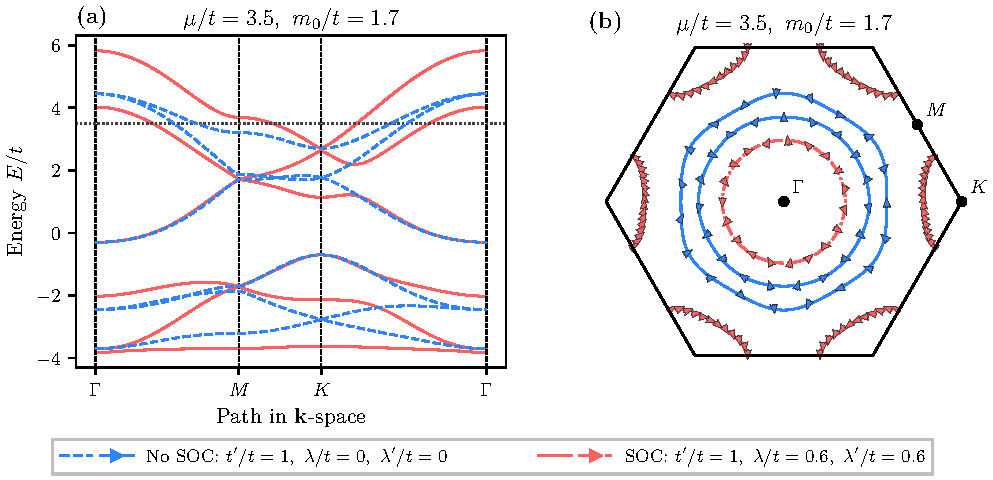
\includegraphics[
        width=\linewidth
    ]{Plots/Mn3Pt T1/Mn3Pt1 nonbreathing.pdf}
    \par\bigskip
    \begin{subfigure}[t]{0.46\textwidth}
        \centering
        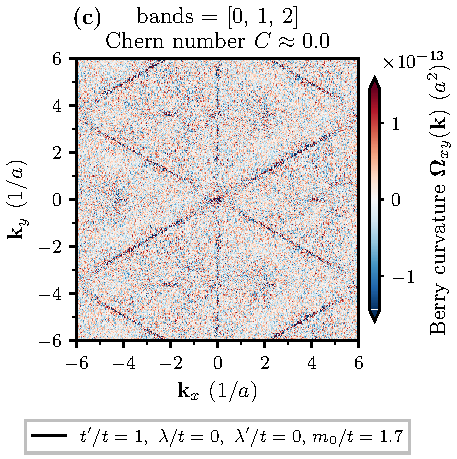
\includegraphics[
            width=\linewidth
        ]{Plots/Mn3Pt T1/Mn3Pt1 nonbreathing_berry_wo_soc.pdf}
        
    \end{subfigure}
    \hfill
    \begin{subfigure}[t]{0.48\textwidth}
        \centering
        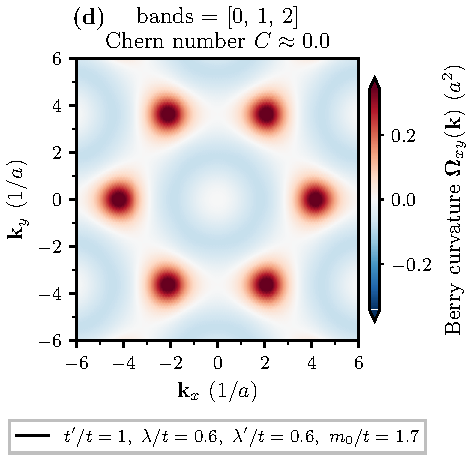
\includegraphics[
            width=\linewidth
        ]{Plots/Mn3Pt T1/Mn3Pt1 nonbreathing_berry_w_soc.pdf}
        
    \end{subfigure}
    \caption{\textbf{Tight-binding results for the T1 phase of \ce{Mn3Pt} in the nonbreathing limit, with the magnetic texture shown in Fig.~\ref{fig: magnetic texture Mn3Pt} (a), obtained using the Bloch Hamiltonian in Eq.~\eqref{eq: bloch-Hamiltonian}.} (a) Electronic band structure along the high-symmetry path $\Gamma$--$M$--$K$. (b) In-plane spin texture on the Fermi surface at the chemical potential $\mu$. (c,d) Berry curvature calculated without and with spin--orbit coupling (SOC), respectively, using the Fukui--Hatsugai--Suzuki method described in Eq.~\eqref{eq: berry curv comp}.}
    \label{fig:Mn3Pt1-nonbreathing}
\end{figure}
This argument does not work for $K$ because $K+\mathbf{G} = -K\neq K$. However, it can be argued by using $[C_{3z}||C_{3z}]$ and evenness in $\mathbf{k}$ that a degeneracy at $K$ is allowed given by 
\begin{align}
    E_n(K) = E_m(-K) = E_\ell(-C_{3z}K) = E_\ell(K'+\mathbf{G}) = E_\ell(K)
    \label{eq: degeneracy_C3z_even_for_K}
\end{align}
with $K' = -K $.
Note that we did not show that $n \neq \ell$ or $n\neq m$ and therefore the symmetry arguments do not prove that this degeneracy occurs. They only provide an explanation for degeneracies that may occur at the given $\mathbf{k}$-points. \\


For the breathing kagome lattice, we expect the $[E||C_{2\hat{z}}]$-symmetry to be broken and therefore the energy, spin and Berry curvature not to be generally even in $\mathbf{k}$, as confirmed in Fig.~\ref{fig:Mn3Pt1-breathing}. However, in the absence of SOC, $\Theta_s[C_{2z}||E]$ still forces the in-plane spins and energies to be even and the Berry curvature to be odd in $\mathbf{k}$, as observed in Fig.~\ref{fig:Mn3Pt1-breathing}. Therefore, even when $[E||C_{2\hat{z}}]$ is broken, the energy and in-plane spins remain even in the absence of SOC. Additionally, the out-of-plane spin component is expected to be odd in $\mathbf{k}$.\\

We also observe a $C_{3z}^s$-symmetry as expected.

% Lastly, we note that the $\mathcal{TM}$-plane is visible for all chosen cases, however, by using numerical calculations, we show, with the use of OpenAI's 'ChatGPT' for helping with the creation of the code, that the $\mathcal{TM}$-symmetry is actually slightly broken for SOC, as expected. \\
% For this, we use $U_{TM} \mathfrak
% {H}(\mathbf{k})^*U_{TM} = \mathfrak
% {H}(-\mathcal{M}\mathbf{k})$ with $U_{{TM}} = P \otimes U_{TM}^{\text{spin}} = P \otimes U_{M}^\text{spin}i\sigma_y\mathcal{K}$, where we use the spatial mirror $P$, assigning the sublattices onto the according position, and the spinful mirror operator $U_\mathcal{M}^\text{spin}$, rotating the spins perpendicular to the mirror plane because of the pseudovectorial characteristics of spins. \\

\begin{figure}[tbhp]
    \centering
    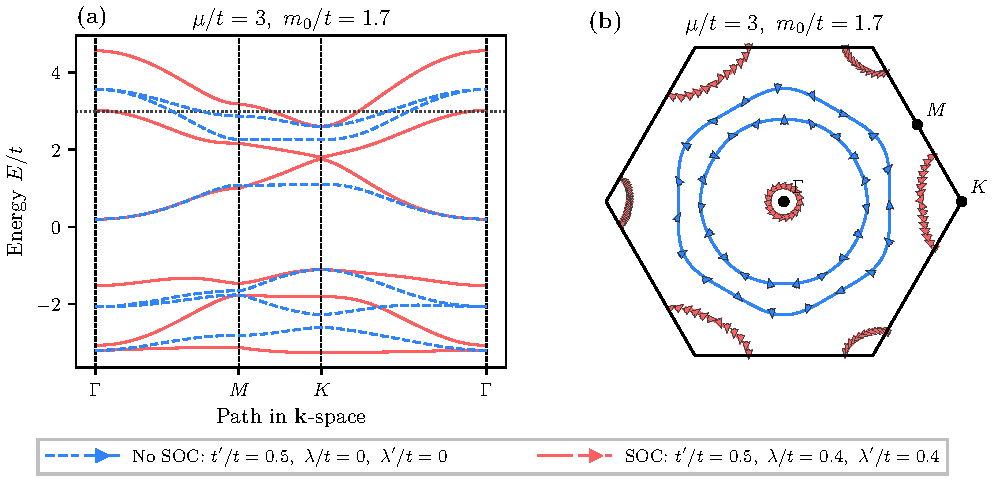
\includegraphics[
        width=\linewidth
    ]{Plots/Mn3Pt T1/Mn3Pt1 breathing.pdf}
    \par\bigskip
    \begin{subfigure}[t]{0.48\textwidth}
        \centering
        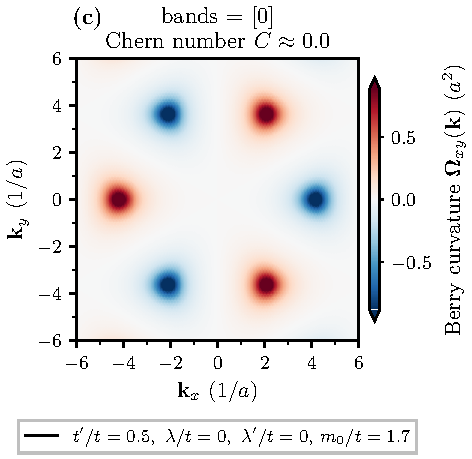
\includegraphics[
            width=\linewidth
        ]{Plots/Mn3Pt T1/Mn3Pt1 breathing_berry_wo_soc.pdf}
        
    \end{subfigure}
    \hfill
    \begin{subfigure}[t]{0.48\textwidth}
        \centering
        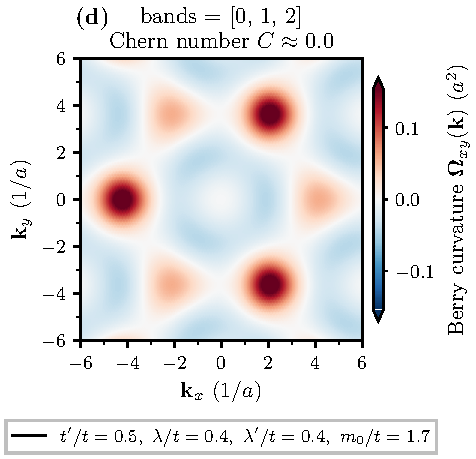
\includegraphics[
            width=\linewidth
        ]{Plots/Mn3Pt T1/Mn3Pt1 breathing_berry_w_soc.pdf}
        
    \end{subfigure}
    \caption{\textbf{Tight-binding results for the T1 phase of \ce{Mn3Pt} in a breathing lattice, with the magnetic texture shown in Fig.~\ref{fig: magnetic texture Mn3Pt} (a), obtained using the Bloch Hamiltonian in Eq.~\eqref{eq: bloch-Hamiltonian}.} (a) Electronic band structure along the high-symmetry path $\Gamma$--$M$--$K$. (b) In-plane spin texture on the Fermi surface at the chemical potential $\mu$. (c,d) Berry curvature calculated without and with spin--orbit coupling (SOC), respectively, using the Fukui--Hatsugai--Suzuki method described in Eq.~\eqref{eq: berry curv comp}.}
    \label{fig:Mn3Pt1-breathing}
\end{figure}

Lastly, we observe $[C_{2\hat{s}}||\sigma_v]$ in the absence of SOC and the $\mathcal{TM}$ planes, depicted in Fig.~\ref{fig: magnetic texture Mn3Pt} (a). The $\mathcal{TM}$-typical behavior is given by Eq.~\eqref{eq: symmetry_TM} and is also observed in a numerical calculation in the presence of SOC. Therefore, we observe our data to be compatible with a $\mathcal{TM}$ symmetry as expected due to a conserved $\mathcal{TM}$ and $C_{3z}^s$ symmetry in the presence of SOC.  
\FloatBarrier
\subsection{Electronic structure of the T2 phase}
Similarly to the T1 phase, we compute the band structure, Fermi-surface spin textures and Berry curvature as depicted in Figs.~\ref{fig:Mn3Pt2-nonbreathing} and \ref{fig:Mn3Pt2-breathing}.
A similar behavior in comparison to the T1 phase is observed. The principal difference is that the T2 phase has $\mathcal{M}$ planes rather than the $\mathcal{TM}$ planes of T1 and an additional global phase shift, as shown in Fig.~\ref{fig: magnetic texture Mn3Pt} (b). 
\\
Similar symmetry arguments for the occurrence of degeneracies, as given in Eqs.~\eqref{eq: degeneracy_C3z_even_for_K},~\eqref{eq: degeneracy_even_for_Gamma} and \eqref{eq: degeneracy_even_for_M}, can be applied to the T2 phase, and therefore degeneracies at $K$, $\Gamma$ and $M$ are permitted if the energy is even in $\mathbf{k}$.

\begin{figure}[tbhp]
    \centering
    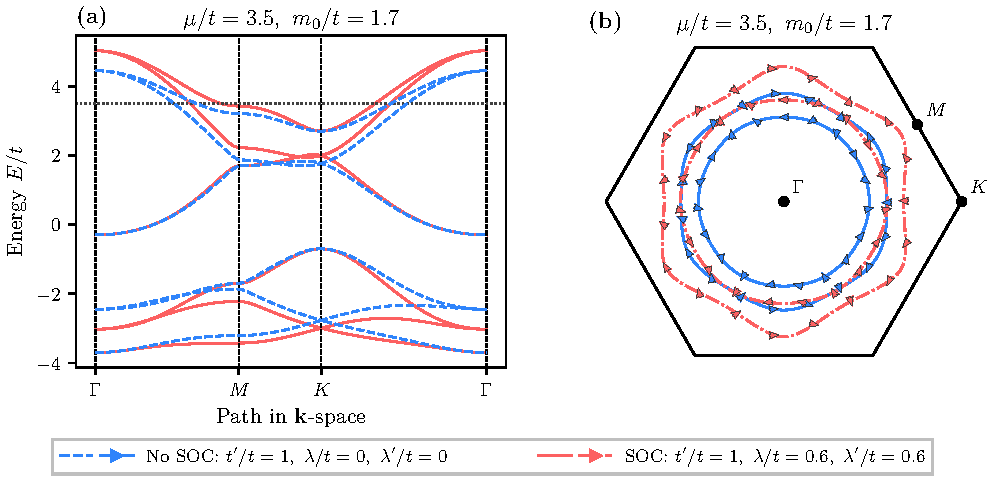
\includegraphics[
        width=\linewidth
    ]{Plots/Mn3Pt T2/Mn3Pt2 nonbreathing.pdf}
    \par\bigskip
    \begin{subfigure}[t]{0.48\textwidth}
        \centering
        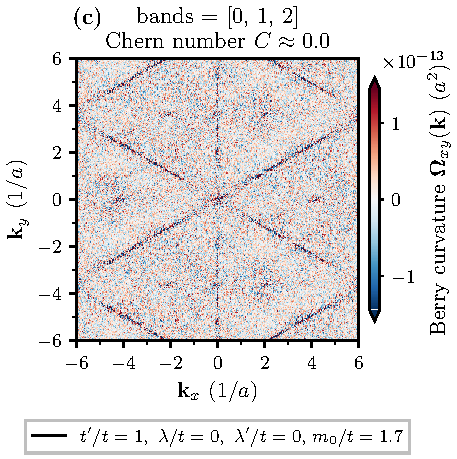
\includegraphics[
            width=\linewidth
        ]{Plots/Mn3Pt T2/Mn3Pt2 nonbreathing_berry_wo_soc.pdf}
        
    \end{subfigure}
    \hfill
    \begin{subfigure}[t]{0.48\textwidth}
        \centering
        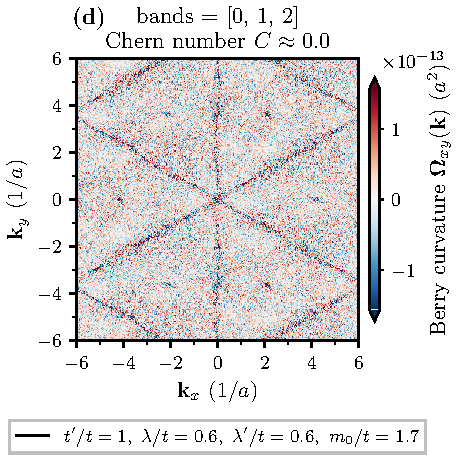
\includegraphics[
            width=\linewidth
        ]{Plots/Mn3Pt T2/Mn3Pt2 nonbreathing_berry_w_soc.pdf}
        
    \end{subfigure}
    \caption{\textbf{Tight-binding results for the T2 phase of \ce{Mn3Pt} in the nonbreathing limit, with the magnetic texture shown in Fig.~\ref{fig: magnetic texture Mn3Pt} (b), obtained using the Bloch Hamiltonian in Eq.~\eqref{eq: bloch-Hamiltonian}.} (a) Electronic band structure along the high-symmetry path $\Gamma$--$M$--$K$. (b) In-plane spin texture on the Fermi surface at the chemical potential $\mu$. (c,d) Berry curvature calculated without and with spin--orbit coupling (SOC), respectively, using the Fukui--Hatsugai--Suzuki method described in Eq.~\eqref{eq: berry curv comp}.}
    \label{fig:Mn3Pt2-nonbreathing}
\end{figure}
The two phases give equivalent results in the absence of SOC, as seen by comparing Figs.~\ref{fig:Mn3Pt1-nonbreathing} and \ref{fig:Mn3Pt2-nonbreathing} or Figs.~\ref{fig:Mn3Pt1-breathing} and \ref{fig:Mn3Pt2-breathing} due to the global spin rotation of $\pi/2$, shown in Fig.~\ref{fig: magnetic texture Mn3Pt}. Therefore, the spin texture is expected to be rotated by an additional global phase of $\pi/2$ for the T2 phase in the absence of SOC.
The Berry curvature vanishes in the mirror-invariant plane $\mathcal{M}$, as observed in Fig.~\ref{fig:Mn3Pt2-breathing}, and the behavior according to Eq.~\eqref{eq: symmetry_M} is observed for energy, in-plane spin and Berry curvature in Figs.~\ref{fig:Mn3Pt2-nonbreathing} and \ref{fig:Mn3Pt2-breathing}. Thus, the mirror plane is observed in the electronic-structure properties. The vanishing of the Berry curvature on the mirror-invariant plane stems from it being odd under the mirror plane. In the Fermi-surface spin textures, the spin on the mirror plane is expected to be perpendicular to the mirror plane. \\
We again observe the $C_{3z}$ behavior and, without SOC, even energies and in-plane spins but an odd Berry curvature, where the former is imposed by $C_{3z}^s$ and the latter by $\Theta_s[C_{2z}||E]$.
Thus, the Berry curvature vanishes in the absence of SOC in the nonbreathing limit. We also observe that the Berry curvature vanishes in the presence of SOC in the nonbreathing limit. Although this result would be consistent with an additional $\mathcal{TM}$ symmetry in the $xz$-plane, which could occur only
in the nonbreathing limit, such a symmetry has not been established for the full Hamiltonian. Therefore, a future study would have to show this. Hence, we treat this as a numerical observation. Nevertheless, independently of the additional symmetry plane, the Chern number is forced to zero due to the conserved $\mathcal{M}$ symmetry.
\begin{figure}[tbhp]
    \centering
    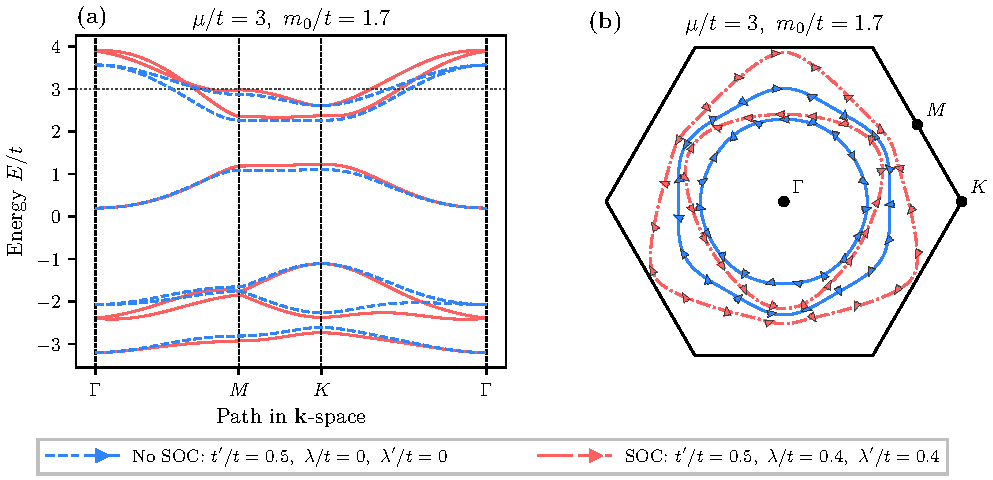
\includegraphics[
        width=\linewidth
    ]{Plots/Mn3Pt T2/Mn3Pt2 breathing.pdf}
    \par\bigskip
    \begin{subfigure}[t]{0.48\textwidth}
        \centering
        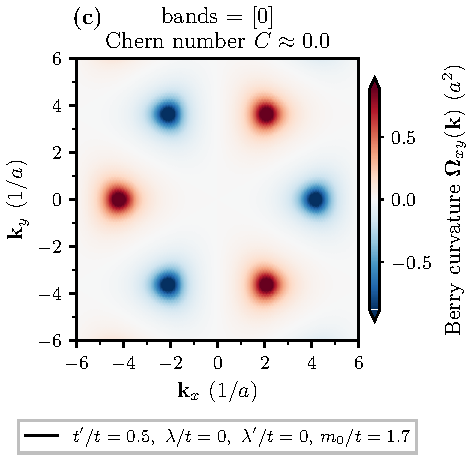
\includegraphics[
            width=\linewidth
        ]{Plots/Mn3Pt T2/Mn3Pt2 breathing_berry_wo_soc.pdf}
        
    \end{subfigure}
    \hfill
    \begin{subfigure}[t]{0.48\textwidth}
        \centering
        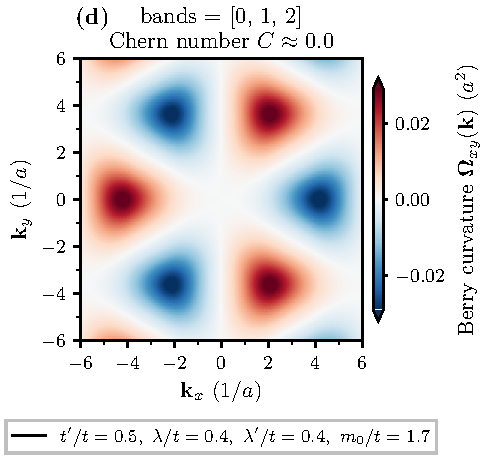
\includegraphics[
            width=\linewidth
        ]{Plots/Mn3Pt T2/Mn3Pt2 breathing_berry_w_soc.pdf}
        
    \end{subfigure}
    \caption{\textbf{Tight-binding results for the T2 phase of \ce{Mn3Pt} in a breathing lattice, with the magnetic texture shown in Fig.~\ref{fig: magnetic texture Mn3Pt} (b), obtained using the Bloch Hamiltonian in Eq.~\eqref{eq: bloch-Hamiltonian}.} (a) Electronic band structure along the high-symmetry path $\Gamma$--$M$--$K$. (b) In-plane spin texture on the Fermi surface at the chemical potential $\mu$. (c,d) Berry curvature calculated without and with spin--orbit coupling (SOC), respectively, using the Fukui--Hatsugai--Suzuki method described in Eq.~\eqref{eq: berry curv comp}.}
    \label{fig:Mn3Pt2-breathing}
\end{figure}

The alternating form of the Berry curvature for a breathing lattice comes from the combination of $C_{3z}^s$ and the mirror plane $\mathcal{M}$. An odd behavior of the Berry curvature is not expected in the presence of SOC, and can be checked numerically by calculating
\begin{align}
\frac{\max_{\mathbf{k}}\left|\Omega_{xy}^{(n)}(\mathbf{k})+\Omega_{xy}^{(n)}(-\mathbf{k})\right|}{\max_{\mathbf{k}}\left|\Omega_{xy}^{(n)}(\mathbf{k})\right|}\approx 0.02, \nonumber
\end{align}
which yields numerical nonzero values and therefore no odd behavior of the Berry curvature.
In the absence of SOC for the breathing case, the energy and in-plane spins are as expected even, whereas the Berry curvature is odd.
\newpage
\section{M-type altermagnetism in \ce{Mn3Ge} and \ce{Mn3Sn}}
In this section, the model and symmetries formulated in Chapter~\ref{chapter:Theory} are applied to the magnetic texture of the M-type altermagnets \ce{Mn3Ge} and \ce{Mn3Sn}. 
Further, the expectations are compared with the computed results of the band structure, in-plane Fermi-surface spin texture and the out-of-plane component of Berry curvature.

\subsection{Magnetic structures and symmetries of \ce{Mn3Ge} and \ce{Mn3Sn}}

Similarly to \ce{Mn3Pt}, a kagome lattice consisting of manganese atoms in \ce{Mn3Ge} and \ce{Mn3Sn} is obtained by projecting the atoms onto the $(0001)$-plane in the hexagonal structure $D0_{19}$, as stated, for example, in Ref.~\cite{10.1063/1.5064697}. Here, the localized magnetic moments reside predominantly on the manganese atoms due to nearly filled orbitals of the $\ce{Ge}$ and $\ce{Sn}$ atoms, thus weak magnetic moments. \\
The magnetic moments form a triangular $120^\circ$ order and therefore the structures depicted in Figs.~\ref{fig: magnetic texture Mn3Ge and Sn}~(a) and (b) are consistent with the magnetic point groups $m'mm'$ and $mm'm'$, respectively.\\
For \ce{Mn3Ge}, the phases of the magnetic texture in Fig.~\ref{fig: magnetic texture Mn3Ge and Sn} are $\varphi_{3,A} = \pi/2$, $\varphi_{3,B} = 11\pi/6$ and $\varphi_{3,C}= 7\pi/6$. The magnetic texture of \ce{Mn3Sn} is obtained by adding a global spin rotation of $\pi/2$ to the magnetic moments.\\

In the magnetic texture, the symmetry $[C_{3z}||C_{3z}^{-1}]$ is found, which combines a $120^\circ$ spin-space rotation and a $-120^\circ$ spatial rotation. This symmetry stems from the magnetic order, depicted in Fig.~\ref{fig: magnetic texture Mn3Ge and Sn}, which can be verified using the relations
\begin{align}
    A\to B & \qquad  \varphi_B = \varphi_A -\frac{2\pi}{3} \nonumber \\
    B\to C & \qquad \varphi_C = \varphi_B -\frac{2\pi}{3} \nonumber  \\
    C\to A & \qquad \varphi_A = \varphi_C -\frac{2\pi}{3}.
\end{align}
Therefore, we expect the relations given by

\begin{align}
    E_m(C_{3z}\mathbf k)&=E_n(\mathbf k) \nonumber\\
    \mathbf s_m(C_{3z}\mathbf k)
  &=C_{3z}^{-1}\mathbf s_n(\mathbf k) \nonumber\\
    \Omega_{xy}^{(m)}(C_{3z}\mathbf k)
  &=\Omega_{xy}^{(n)}(\mathbf k),
    \label{eq: C_3z^-1 symm}
\end{align}
analogous to Eq.~\eqref{eq: C_3z^s symm}, in the absence of SOC. The symmetry breaks in the presence of SOC, due to inequivalent transformations for spin- and real-space.
The symmetry also fixes the in-plane net magnetization to zero, analogously to $C_{3z}^s$ for \ce{Mn3Pt}, in the absence of SOC.

The $\mathcal{M}$ and $\mathcal{TM}$ planes depicted in Fig.~\ref{fig: magnetic texture Mn3Ge and Sn} impose the constraints in Eq.~\eqref{eq: symmetry_M} and \eqref{eq: symmetry_TM}.
The conservation of the $\mathcal{M}$ and $\mathcal{TM}$ symmetries in the presence of SOC is shown in Section~\ref{section: Symmetries}. 
Additionally, we argue that the mirror plane $\mathcal{M}$, which is in this case equal to $[C_{2\hat{s}}||\sigma_v]$ because the spin is perpendicular to the mirror plane, is preserved in the presence of SOC due to $[C_{2\hat{s}}||\sigma_v]$ transforming spin-space and real-space equivalently.
Thus, the $\mathcal{M}$ and $\mathcal{TM}$ planes are expected to be visible in the presence of SOC.

In contrast, the $[C_{2\hat{\mathbf{s}}}||\sigma_v]$ operator, whose plane is depicted in Fig.~\ref{fig: magnetic texture Mn3Ge and Sn}, is broken by SOC in \ce{Mn3Ge} because the spin at the mirror-invariant site lies within the mirror plane, therefore, the spin-space and spatial transformations are inequivalent.   \\


%NEEEL TEMPERATURE https://www.sciencedirect.com/science/article/abs/pii/S0304885322009039 365K - 400K!!!

\begin{figure}[tbhp]
    \centering
    % First Subfigure
    \begin{subfigure}[c]{0.48\textwidth}
        \centering
        \begin{tikzpicture}[scale=1.5]
        
          % half-length of each spin arrow
          \def\spinhalf{0.3}
        
          % angles of the three sublattices
          \def\phiA{90}
          \def\phiB{330}
          \def\phiC{210}
        
          % useful constants
          \pgfmathsetmacro{\rt}{sqrt(3)}
          \pgfmathsetmacro{\rthalf}{sqrt(3)/2}
        
          % lattice
          \draw[very thick, dashed]
            (0,0) -- (0.5,\rthalf) -- (1.5,\rthalf) -- (2,0)
            -- (1.5,-\rthalf) -- (0.5,-\rthalf) -- (0,0)
            -- (-0.5,\rthalf) -- (0.5,\rthalf) -- (1,\rt)
            -- (1.5,\rthalf) -- (2.5,\rthalf) -- (2,0)
            -- (2.5,-\rthalf) -- (1.5,-\rthalf) -- (1,-\rt)
            -- (0.5,-\rthalf) -- (-0.5,-\rthalf) -- (0,0);
            
          \draw[thick, brown] (1,{4*sqrt(3)/3}) -- (1,{-4*sqrt(3)/3}) node[below, font=\small]{$\mathcal{TM}$, $\sigma_v$};
          % sublattice A
          \foreach \x/\y in {
            1/{-\rt},
            0/0,
            1/{\rt},
            2/0
          }{
            \centerspin[pastelblue]{(\x,\y)}{\phiA}
          }
        
          % sublattice B
          \foreach \x/\y in {
            0.5/{\rthalf},
            1.5/{-\rthalf},
            -0.5/{-\rthalf},
            2.5/{\rthalf}
          }{
            \centerspin[pastelred]{(\x,\y)}{\phiB}
          }
        
          % sublattice C
          \foreach \x/\y in {
            0.5/{-\rthalf},
            1.5/{\rthalf},
            -0.5/{\rthalf},
            2.5/{-\rthalf}
          }{
            \centerspin[pastelgreen]{(\x,\y)}{\phiC}
          }

        \end{tikzpicture}
    \caption{\ce{Mn3Ge}}
    \label{fig: magnetic texture Mn3Ge}
    \end{subfigure}
    \begin{subfigure}[c]{0.48\textwidth}
    \centering
    \begin{tikzpicture}[scale=1.5]
    
      % half-length of each spin arrow
      \def\spinhalf{0.3}
    
      % angles of the three sublattices
      \def\phiA{0}
      \def\phiB{240}
      \def\phiC{120}
    
      % useful constants
      \pgfmathsetmacro{\rt}{sqrt(3)}
      \pgfmathsetmacro{\rthalf}{sqrt(3)/2}
    
      % lattice
      \draw[very thick, dashed]
        (0,0) -- (0.5,\rthalf) -- (1.5,\rthalf) -- (2,0)
        -- (1.5,-\rthalf) -- (0.5,-\rthalf) -- (0,0)
        -- (-0.5,\rthalf) -- (0.5,\rthalf) -- (1,\rt)
        -- (1.5,\rthalf) -- (2.5,\rthalf) -- (2,0)
        -- (2.5,-\rthalf) -- (1.5,-\rthalf) -- (1,-\rt)
        -- (0.5,-\rthalf) -- (-0.5,-\rthalf) -- (0,0);
          \draw[thick, brown] (1,{4*sqrt(3)/3}) -- (1,{-4*sqrt(3)/3}) node[below, font=\small]{$\mathcal{M}$, $\sigma_v$};
      % sublattice A
      \foreach \x/\y in {
        1/{-\rt},
        0/0,
        1/{\rt},
        2/0
      }{
        \centerspin[pastelblue]{(\x,\y)}{\phiA}
      }
    
      % sublattice B
      \foreach \x/\y in {
        0.5/{\rthalf},
        1.5/{-\rthalf},
        -0.5/{-\rthalf},
        2.5/{\rthalf}
      }{
        \centerspin[pastelred]{(\x,\y)}{\phiB}
      }
    
      % sublattice C
      \foreach \x/\y in {
        0.5/{-\rthalf},
        1.5/{\rthalf},
        -0.5/{\rthalf},
        2.5/{-\rthalf}
      }{
        \centerspin[pastelgreen]{(\x,\y)}{\phiC}
      }

    
    \end{tikzpicture}
    \caption{\ce{Mn3Sn}}
    \label{fig: magnetic texture Mn3Sn}
    \end{subfigure}
    \caption{The magnetic order of (a) \ce{Mn3Ge} and (b) \ce{Mn3Sn}, as defined in Ref. \cite{Quelle1}, with the illustrated time-reversal mirror plane $\mathcal{TM}$ or mirror plane $\mathcal{M}$, respectively, and the reflection symmetry $\sigma_v$, belonging to $[C_{2\hat{s}}||\sigma_v]$, depicted on the corresponding kagome lattice. The magnetic order of \ce{Mn3Ge} has a time-reversal mirror plane, whereas that of \ce{Mn3Sn} has a mirror plane.}
    \label{fig: magnetic texture Mn3Ge and Sn}
\end{figure}

By analogy with \ce{Mn3Pt}, the symmetries $\Theta_s [C_{2z}||E]$ and $[E||C_{2z}]$ are expected, where the former holds in the absence of SOC and the latter in the nonbreathing limit. 
Also, the two textures are predicted to behave identically in the absence of SOC with respect to the global spin rotation of $\pi/2$.\\
These symmetries constrain the direction of an allowed magnetization. When $[C_{3z}||C_{3z}^{-1}]$ is broken by adding SOC, a net magnetization is permitted in \ce{Mn3Ge} within the $\mathcal{TM}$ plane, i.e., along the $y$-axis, and in \ce{Mn3Sn} perpendicular to the $\mathcal{M}$ plane, i.e., along the $x$-axis.  



\subsection{Electronic structure of \ce{Mn3Ge}}
The computed band structure, in-plane Fermi-surface spin texture and Berry curvature are shown in Fig.~\ref{fig:Mn3Ge-nonbreathing} for the nonbreathing limit and in Fig.~\ref{fig:Mn3Ge-breathing} for a breathing kagome lattice.
\begin{figure}[tbhp]
    \centering
    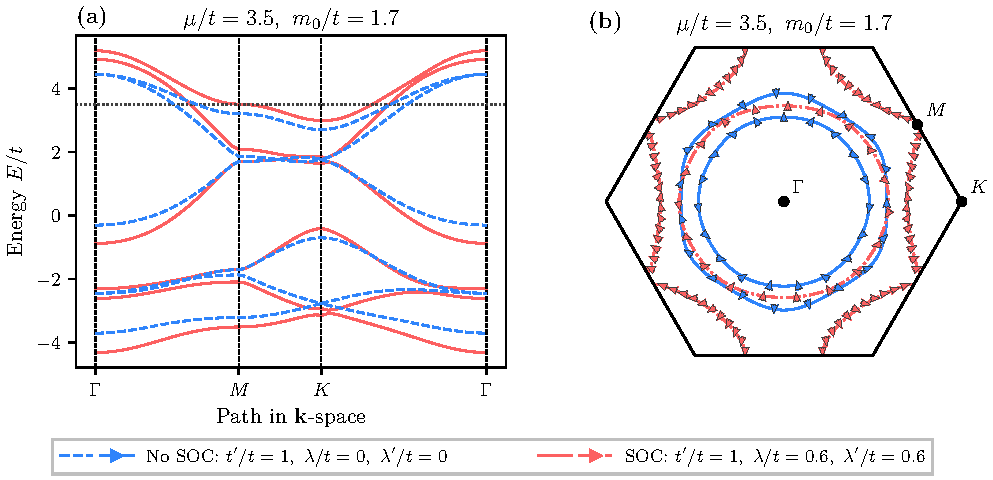
\includegraphics[
        width=\linewidth
    ]{Plots/Mn3Ge/Mn3Ge nonbreathing.pdf}
    \par\bigskip
    \begin{subfigure}[t]{0.46\textwidth}
        \centering
        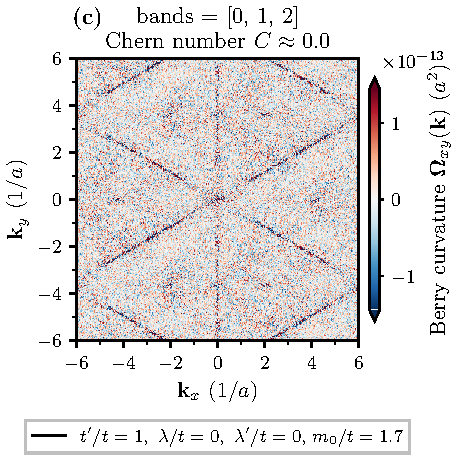
\includegraphics[
            width=\linewidth
        ]{Plots/Mn3Ge/Mn3Ge nonbreathing_berry_wo_soc.pdf}
        
    \end{subfigure}
    \hfill
    \begin{subfigure}[t]{0.48\textwidth}
        \centering
        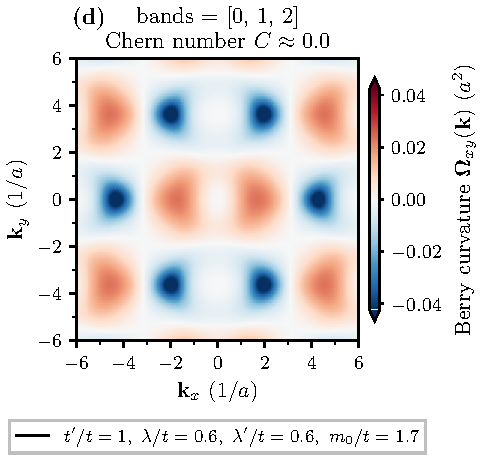
\includegraphics[
            width=\linewidth
        ]{Plots/Mn3Ge/Mn3Ge nonbreathing_berry_w_soc.pdf}
        
    \end{subfigure}
    \caption{\textbf{Tight-binding results for \ce{Mn3Ge} in the nonbreathing limit, with the magnetic texture shown in Fig.~\ref{fig: magnetic texture Mn3Ge and Sn}~(a), obtained using the Bloch Hamiltonian in Eq.~\eqref{eq: bloch-Hamiltonian}.} (a) Electronic band structure along the high-symmetry path $\Gamma$--$M$--$K$. (b) In-plane spin texture on the Fermi surface at the chemical potential $\mu$. (c,d) Berry curvature calculated without and with spin--orbit coupling (SOC), respectively, using the Fukui--Hatsugai--Suzuki method described in Eq.~\eqref{eq: berry curv comp}.}
\label{fig:Mn3Ge-nonbreathing}
\end{figure}
For the nonbreathing limit, the Berry curvature, energies, and spins are
even in $\mathbf{k}$, as imposed by $[E||C_{2z}]$, which also holds in the presence of SOC.\\
This operation and the $\Theta_s [C_{2z}||E]$ operator in the nonbreathing limit in the absence of SOC lead to a vanishing Berry curvature as seen in Fig.~\ref{fig:Mn3Ge-nonbreathing} (c), as also confirmed for \ce{Mn3Pt}. The imposed properties of $[C_{3z}||C_{3z}^{-1}]$, given by Eq.~\eqref{eq: C_3z^-1 symm}, are observed in the absence of SOC in Figs.~\ref{fig:Mn3Ge-nonbreathing} and \ref{fig:Mn3Ge-breathing}, therefore confirming the prediction. In the presence of SOC, $[C_{3z}||C_{3z}^{-1}]$ breaks. Thus, in the presence of SOC, the evenness, imposed by $[E||C_{2z}]$, is expected, as observed in Fig.~\ref{fig:Mn3Ge-nonbreathing}. \\
The properties imposed by $[C_{2\hat{s}}||\sigma_v]$ can also be observed in the absence of SOC. We are also able to observe properties imposed by the $\mathcal{TM}$ plane, according to Eq.~\eqref{eq: symmetry_TM}, in the case of SOC. Therefore, matching with our previously established expectations. \\

% The obtained results show a conservation of the $\mathcal{TM}$ plane for SOC of different orders using Eq.~\eqref{eq: TM symmetry prove eq}. \\
% It might be expected that this breakage is small enough for numerical errors to overtake. 
% Therefore, we are not able to confirm our theory for this case. !!!!!!!!!!!!!!!!!!!
% In Ref. \cite{MnPtSOC} it was confirmed, that the magnetic texture with SOC can be seen to get an out-of plane virtual texture and therefore breaking the $\mathcal{TM}$ plane. The angle of the virtual magnetic texture experiences a change of $\SI{0.15}{\degree}$, which confirms the seemingly holding $\mathcal{TM}$ plane. 
% !!!
\begin{figure}[tbhp]
    \centering
    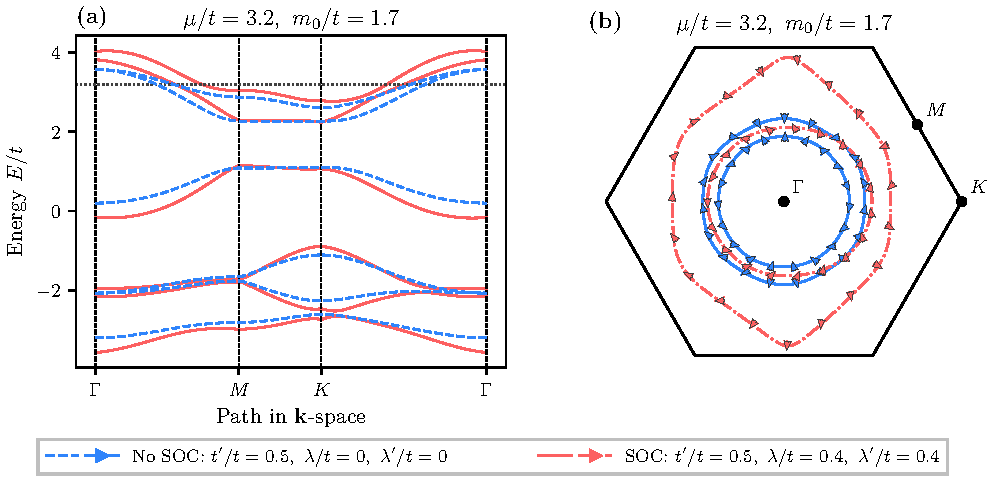
\includegraphics[
        width=\linewidth
    ]{Plots/Mn3Ge/Mn3Ge breathing.pdf}
    \par\bigskip
    \begin{subfigure}[t]{0.48\textwidth}
        \centering
        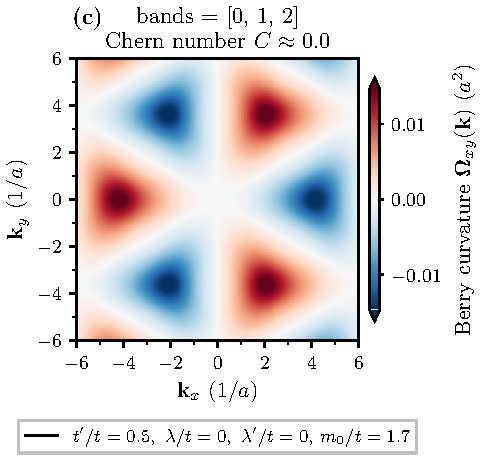
\includegraphics[
            width=\linewidth
        ]{Plots/Mn3Ge/Mn3Ge breathing_berry_wo_soc.pdf}
        
    \end{subfigure}
    \hfill
    \begin{subfigure}[t]{0.48\textwidth}
        \centering
        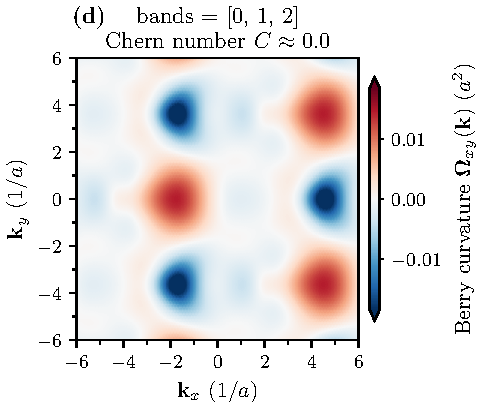
\includegraphics[
            width=\linewidth
        ]{Plots/Mn3Ge/Mn3Ge breathing_berry_w_soc.pdf}
        
    \end{subfigure}
    \caption{\textbf{Tight-binding results for \ce{Mn3Ge} in the breathing lattice, with the magnetic texture shown in Fig.~\ref{fig: magnetic texture Mn3Ge and Sn}~(a), obtained using the Bloch Hamiltonian in Eq.~\eqref{eq: bloch-Hamiltonian}.} (a) Electronic band structure along the high-symmetry path $\Gamma$--$M$--$K$. (b) In-plane spin texture on the Fermi surface at the chemical potential $\mu$. (c,d) Berry curvature calculated without and with spin--orbit coupling (SOC), respectively, using the Fukui--Hatsugai--Suzuki method described in Eq.~\eqref{eq: berry curv comp}.}
    \label{fig:Mn3Ge-breathing}
\end{figure}
Breaking the nonbreathing limit by introducing unequal hopping parameters breaks
the symmetry $[E||C_{2z}]$ that otherwise imposes evenness, thereby allowing a nonzero Berry curvature in the absence of SOC, which was earlier prohibited by $\Theta_s[C_{2z}||E]$ and $[E||C_{2z}]$. Therefore, we are able to observe the odd behavior of the Berry curvature, imposed by $\Theta_s [C_{2z}||E]$, forcing the total Chern number of an isolated composite subspace to vanish, as seen in Fig.~\ref{fig:Mn3Ge-breathing}~(c). \\
The energy and spins are even in the absence of SOC, whereas the Berry curvature is odd, due to $\Theta_s[C_{2z}||E]$. These constraints, together with $[C_{3z}||C_{3z}^{-1}]$ and the $\mathcal{TM}$ plane, lead to the observed behavior in Fig.~\ref{fig:Mn3Ge-breathing}.\\
In the presence of SOC in the breathing lattice, $\Theta_s [C_{2z}||E]$, $[C_{2\hat{s}}||\sigma_v]$ and $[C_{3z}||C_{3z}^{-1}]$ are broken. The only observable properties are the imposed constraints of the $\mathcal{TM}$ symmetry, given by Eq.~\eqref{eq: symmetry_TM}. Thus, the resulting numerical data are compatible with the expected $\mathcal{TM}$ symmetry, conserved in the presence of SOC.\\

In \ce{Mn3Ge}, a net magnetization along the $\mathcal{TM}$ plane, or along $y$, can be formed in the presence of SOC. This is because $[C_{3z}||C_{3z}^{-1}]$ is broken, which allows an in-plane net magnetization, and the $\mathcal{TM}$ plane itself forces the perpendicular component, or, the net magnetization along $x$, to vanish. Thus, a net magnetization is allowed in the $y$-direction. \\
The effects of the resulting net magnetization can be observed in the Fermi-surface spin texture in Figs.~\ref{fig:Mn3Ge-nonbreathing} and \ref{fig:Mn3Ge-breathing} in the case of SOC. We next discuss the origin of the deformation of the Fermi surface. The symmetry plane constrains spins along $k_y=0$ to align along $y$ or with the net magnetization. Using the Rashba term, according to Eq.~\eqref{eq: Rashba_Hamiltonian_standard} and evaluating its expectation value with the eigenstates, we obtain
\begin{align}
    \Delta E_{\text{R},n}=\alpha_{\mathrm R}k_x\langle\sigma_y\rangle_n.
\end{align}
Therefore, opposite $y$-directed spin expectation values experience an energy shift of opposite sign, producing a deformation along $k_x$, as observed in Figs.~\ref{fig:Mn3Ge-nonbreathing} and \ref{fig:Mn3Ge-breathing}.
Thus, Rashba coupling produces a deformation in the Fermi surface perpendicular to the magnetization.


Figs.~\ref{fig:Mn3Ge-nonbreathing} and \ref{fig:Mn3Ge-breathing} show that the bands are spin-split also in the absence of SOC, classifying \ce{Mn3Ge} as a strong altermagnet. The spin-splitting arises because the compensated texture breaks $\mathcal{PT}$ symmetry and other symmetries that would enforce band degeneracies.


Hence, \ce{Mn3Ge} is an altermagnet and permits a weak net magnetization allowed by SOC. Therefore, \ce{Mn3Ge} can be classified as an M-type altermagnet, as confirmed in Ref.~\cite{Cheong2025}.



\subsection{Electronic structure of \ce{Mn3Sn}}
Lastly, we compute the electronic-structure properties in momentum space for \ce{Mn3Sn}, shown in Figs.~\ref{fig:Mn3Sn-nonbreathing} and \ref{fig:Mn3Sn-breathing}.
Because the textures of \ce{Mn3Ge} and \ce{Mn3Sn} are related by a global spin rotation, similarities are expected in the absence of SOC. The change in the magnetic texture leads to a mirror plane $\mathcal{M}$, or analogously $[C_{2\hat{s}}||\sigma_v]$, instead of the $\mathcal{TM}$ plane. The mirror plane imposes the properties given by Eq.~\eqref{eq: symmetry_M}.\\ 
The cases without SOC will not be discussed in detail because we expect equivalent results related by a global spin rotation of $-\pi/2$, which we confirm by comparing Figs.~\ref{fig:Mn3Ge-nonbreathing} and \ref{fig:Mn3Sn-nonbreathing} or Figs.~\ref{fig:Mn3Ge-breathing} and \ref{fig:Mn3Sn-breathing} without SOC. \\




\begin{figure}[htbp]
    \centering
    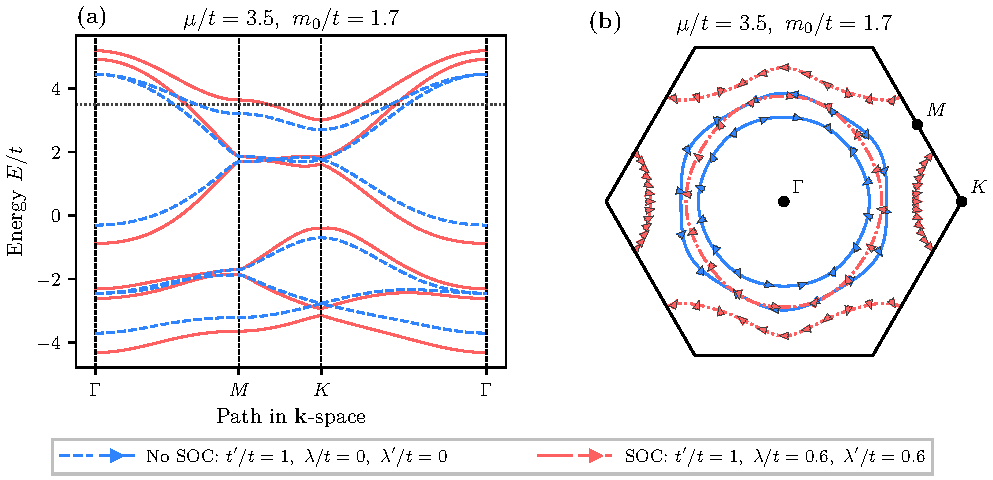
\includegraphics[
        width=\linewidth
    ]{Plots/Mn3Sn/Mn3Sn nonbreathing.pdf}
    \par\bigskip
    \begin{subfigure}[t]{0.46\textwidth}
        \centering
        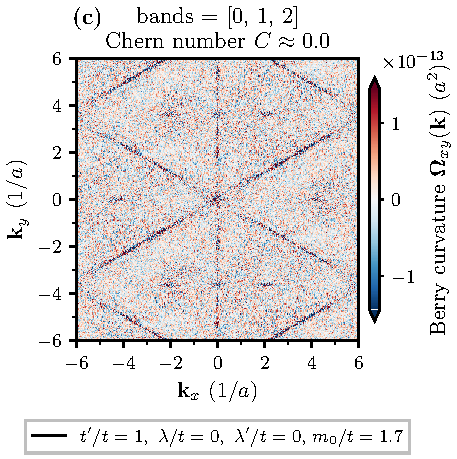
\includegraphics[
            width=\linewidth
        ]{Plots/Mn3Sn/Mn3Sn nonbreathing_berry_wo_soc.pdf}
        
    \end{subfigure}
    \hfill
    \begin{subfigure}[t]{0.48\textwidth}
        \centering
        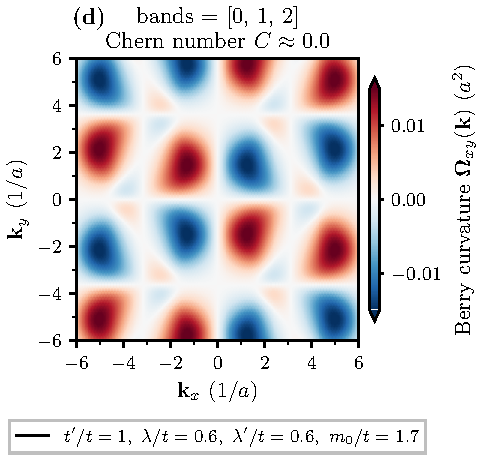
\includegraphics[
            width=\linewidth
        ]{Plots/Mn3Sn/Mn3Sn nonbreathing_berry_w_soc.pdf}
        
    \end{subfigure}
    \caption{\textbf{Tight-binding results for \ce{Mn3Sn} in the nonbreathing limit, with the magnetic texture shown in Fig.~\ref{fig: magnetic texture Mn3Ge and Sn}~(b), obtained using the Bloch Hamiltonian in Eq.~\eqref{eq: bloch-Hamiltonian}.} (a) Electronic band structure along the high-symmetry path $\Gamma$--$M$--$K$. (b) In-plane spin texture on the Fermi surface at the chemical potential $\mu$. (c,d) Berry curvature calculated without and with spin--orbit coupling (SOC), respectively, using the Fukui--Hatsugai--Suzuki method described in Eq.~\eqref{eq: berry curv comp}.}
    \label{fig:Mn3Sn-nonbreathing}
\end{figure}
In the nonbreathing limit, in the presence of SOC, we are able to observe the constraints given by the $\mathcal{M}$ plane, which force the spins to align perpendicular to it  on the mirror-invariant momentum line and the Berry curvature to vanish on it. A mirror-symmetric Fermi-surface spin texture can be seen in Fig.~\ref{fig:Mn3Sn-nonbreathing} (b).
In the nonbreathing limit, we expect the $[E||C_{2z}]$-symmetry, imposing evenness in the electronic-structure energy, spins and Berry curvature. \\
Note that none of the constraints imposed by the symmetry $[C_{3z}||C^{-1}_{3z}]$ according to Eq.~\eqref{eq: C_3z^-1 symm} can be observed in the presence of SOC, which is consistent with the found $[C_{3z}||C_{3z}^{-1}]$ symmetry breaking in the presence of SOC. 
\begin{figure}[htbp]
    \centering
    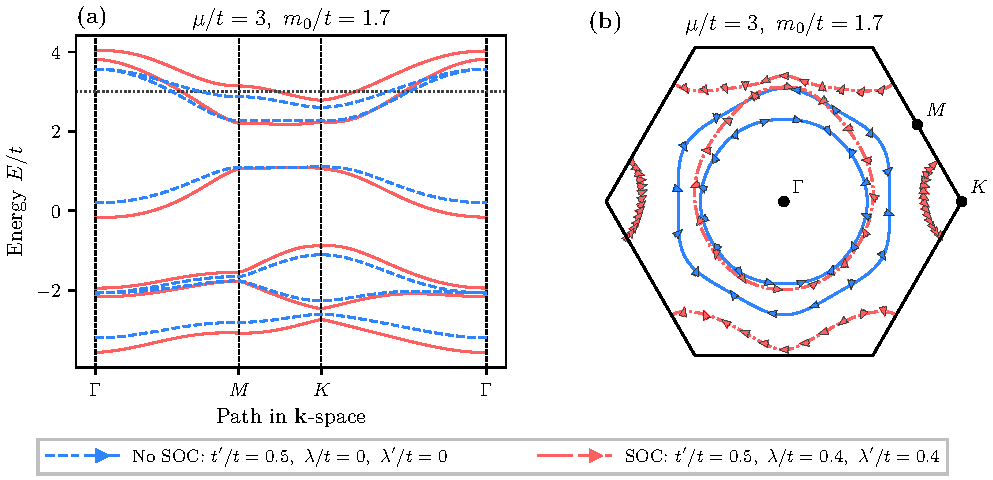
\includegraphics[
        width=\linewidth
    ]{Plots/Mn3Sn/Mn3Sn breathing.pdf}
    \par\bigskip
    \begin{subfigure}[t]{0.48\textwidth}
        \centering
        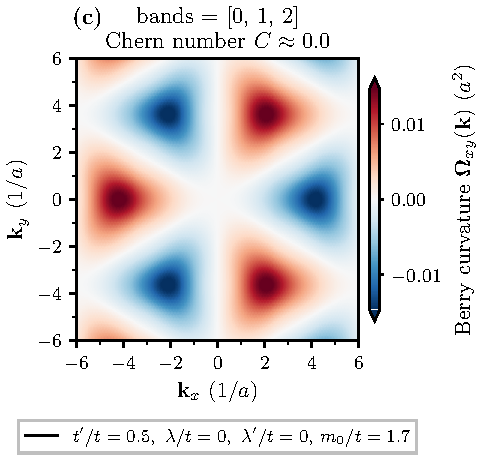
\includegraphics[
            width=\linewidth
        ]{Plots/Mn3Sn/Mn3Sn breathing_berry_wo_soc.pdf}
        
    \end{subfigure}
    \hfill
    \begin{subfigure}[t]{0.48\textwidth}
        \centering
        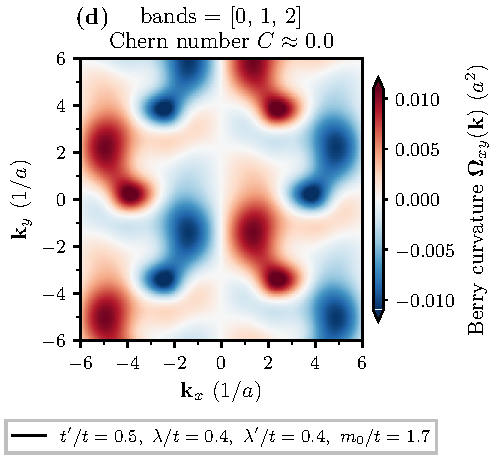
\includegraphics[
            width=\linewidth
        ]{Plots/Mn3Sn/Mn3Sn breathing_berry_w_soc.pdf}
        
    \end{subfigure}
    \caption{\textbf{Tight-binding results for \ce{Mn3Sn} in the breathing lattice, with the magnetic texture shown in Fig.~\ref{fig: magnetic texture Mn3Ge and Sn}~(b), obtained using the Bloch Hamiltonian in Eq.~\eqref{eq: bloch-Hamiltonian}.} (a) Electronic band structure along the high-symmetry path $\Gamma$--$M$--$K$. (b) In-plane spin texture on the Fermi surface at the chemical potential $\mu$. (c,d) Berry curvature calculated without and with spin--orbit coupling (SOC), respectively, using the Fukui--Hatsugai--Suzuki method described in Eq.~\eqref{eq: berry curv comp}.}
    \label{fig:Mn3Sn-breathing}
\end{figure}
Switching to a breathing kagome lattice, the symmetry $[E||C_{2z}]$ is broken, so no longer enforcing evenness. The mirror plane $\mathcal{M}$ perpendicular to the $x$-axis is evident from the vanishing Berry curvature in Fig.~\ref{fig:Mn3Sn-breathing} (d) and in the in-plane Fermi-surface spin texture in Fig.~\ref{fig:Mn3Sn-breathing} (b). The property in Eq.~\eqref{eq: symmetry_M} can also be confirmed by rotating the spins around the $x$-axis and mapping them to the reflected momentum. The only observable symmetry is $\mathcal{M}$ in the presence of SOC and breathing, which is preserved by the system.\\

The mirror plane forces the net magnetization to vanish along  the $y$- and $z$-directions. Analogously to \ce{Mn3Ge}, the broken $[C_{3z}||C_{3z}^{-1}]$ symmetry in the presence of SOC allows an in-plane net magnetization. Thus, an $x$-directed net magnetization is allowed. 

The magnetic order is fully compensated because the three equal-magnitude moments separated by $120^\circ$ sum to zero, as depicted in Fig.~\ref{fig: magnetic texture Mn3Ge and Sn}~(b). 
\ce{Mn3Sn} exhibits spin-split bands also in the absence of SOC. Thus, with full compensation and the spin-split bands, \ce{Mn3Sn} is classified as a strong altermagnet. 
Hence, \ce{Mn3Sn} is a strong altermagnet of M-type, like \ce{Mn3Ge}, exhibiting an $x$-directed net magnetization in the presence of SOC. Therefore, our result agrees with the classification given in Ref.~\cite{Cheong2025}.\\
The effects of the net magnetization can also be seen in the in-plane Fermi-surface spin textures for $k_x=0$, shown in Figs.~\ref{fig:Mn3Sn-nonbreathing} and \ref{fig:Mn3Sn-breathing}, in the presence of SOC. 
Analogously to \ce{Mn3Ge}, we show the effect of magnetization on the Fermi surface.
In the presence of SOC, the Fermi-surface spin textures in Figs.~\ref{fig:Mn3Sn-nonbreathing} and \ref{fig:Mn3Sn-breathing} exhibit a deformation along $k_y$. The mirror symmetry constrains the spins on the mirror plane $k_x=0$ to point along the $x$-direction. Therefore, the energy shift of the Rashba term, obtained by taking its expectation value, is $\Delta E_n=-\alpha_{\mathrm R}k_y\langle\sigma_x\rangle_n$, leading to an increase or decrease of the spin-split energy, depending on the sign of the spin expectation value. This deformation of the Fermi surface is observed.
 
Thus, the net magnetization supports the classification of \ce{Mn3Sn} as an M-type altermagnet, as defined in Ref.~\cite{Cheong2025}.

\chapter{Conclusion and Outlook}
\label{chapter: conclusion}

In this work, we used a tight-binding model on a kagome lattice with different magnetic textures of noncollinear altermagnets. The model includes next-nearest neighbor hopping, Rashba-SOC and a coplanar magnetic exchange texture.\\
Further, we introduced symmetries contained for the magnetic order and the system, applying them on the band structure, in-plane Fermi-surface spin texture and Berry curvature. Then, numerical computations were used to verify the introduced symmetries.\\

In the absence of SOC we find the symmetry $\Theta_s[C_{2z}||E]$, constraining energies, in-plane spins to be even in momentum, while the out-of-plane spin component and Berry curvature are odd.\\
Additionally, in the nonbreathing limit the symmetry $[E||C_{2z}$ was found, imposing evenness in momenutm, thus forcing the Berry curvature to vanish in absence of SOC.\\
Symmetries in the presence of Rashba-SOC break, if the real-space and spin-space transformations are performed independently.\\
Nevertheless, mirror planes $\mathcal{M}$ and time-reversal planes $\mathcal{TM}$ in the $yz$ plane are found to hold even in the presence of SOC. Thus, they enforce constraints on the Fermi-surface spin texture and Berry curvature, which is observed in our numerical observations.\\
While the T1 phase of \ce{Mn3Pt} contains $\mathcal{TM}$ planes, contains the T2 phase an $\mathcal{M}$ plane, which are related by a global spin rotation in the absence of SOC.\\
Similarly, the magnetic textures of \ce{Mn3Ge} and \ce{Mn3Sn} lead to time-reversal mirror and mirror symmetries, respectively, which are again related by a global spin rotation. \\
Due to the global spin rotation in the absence of SOC, we obtain similar results with respect to the global phase shift.\\
Lastly, we found for \ce{Mn3Pt} the $[C_{3z}||C_{3z}]$ symmetry, holding also in the presence of SOC, while for \ce{Mn3Ge} and \ce{Mn3Sn} $[C_{3z}||C_{3z}^{-1}]$ was shown. Thus, \ce{Mn3Pt} exhibits no in-plane net magnetization, whild \ce{Mn3Ge} and \ce{Mn3Sn} can exhibit one along the directions constrained by the $\mathcal{TM}$ and $\mathcal{M}$ planes in the presence of SOC, respectively.\\
Thus, we classify \ce{Mn3Pt} as an S-type altermagnet and \ce{Mn3Ge} and \ce{Mn3Sn} as an altermagnet of M-type.\\
The calculated Berry curvature and spin textures support our introduced symmetry constraints.\\

In this thesis, we used a simple tight-binding model, to easily create a theory about different symmetries. The model includes nearest-neighbor hopping and a precisely coplanar magnetic texture, neglecting next-nearest-neighbor hopping, and further hopping terms, and intrinsic spin-orbit coupling.
Furthermore, we used parameters, which were not obtained by a detailed analysis, thus the results need to be interpreted as an qualitative adaptation of the model onto different magnetic textures.\\

In a subsequent work, the model could be extended by including intrinsic spin-orbit coupling, adding further-neighbor hopping terms or applying it onto non-coplanar textures.
For the latter, an analysis regarding the $\mathcal{TM}$ and $\mathcal{M}$ planes would be interesting, similarly done for the in-plane $\mathcal{TM}$ plane in Ref.\cite{MnPtSOC}.\\



\FloatBarrier



\newpage

\clearpage
\appendix
\chapter{Appendix}
\section{Simplification for the hopping Hamiltonian $H_\text{hop.}$}
\label{chapter: AppendixA}

To further simplify the hopping Hamiltonian $H_\text{hop.}$, we begin by showing 
\begin{align}
    (\mathbf{d}_i \cdot\bm{\hat{\sigma}})^2 &= (d_x \hat{\sigma}_x + d_y \hat{\sigma}_y + d_z \hat{\sigma}_z)^2 \nonumber\\
    &= (d_x^2 + d_y^2 + d_z^2)\hat{I}_2 + d_xd_y\{\hat{\sigma}_x , \hat{\sigma}_y\} + d_yd_z\{\hat{\sigma}_y , \hat{\sigma}_z\} + d_xd_z\{\hat{\sigma}_x , \hat{\sigma}_z\} = \hat{I}_2,
\end{align}
where $\hat{I}_2$ denotes the two-dimensional identity matrix, following from basic operations with the Pauli matrices, where $\{\hat{A} , \hat{B}\} = \hat{A}\hat{B}+\hat{B}\hat{A}$, $|d_i| = 1$ and $\{\hat{\sigma}_i, \hat{\sigma}_j\} = 2\delta_{ij}\hat{I}_2$.
Next, we can use Euler's formula 
\begin{align}
    e^{i\Phi(\mathbf{d}_i\cdot\bm{\hat{\sigma}})} &= \sum_k \frac{(i\Phi)^{2k}}{(2k)!}\hat{I}_3 + \sum_k  \frac{(i\Phi)^{2k+1}}{(2k+1)!} (\mathbf{d}_i\cdot\bm{\hat{\sigma}}) = \cos(\Phi)\hat{I}_2 + i \sin(\Phi) (\mathbf{d}_i\cdot\bm{\hat{\sigma}})\nonumber\\
    &= \frac{1}{\sqrt{t^2+ \lambda^2}}\left\{t\hat{I}_2 - i\lambda (\bm{d}_i \cdot \bm{\hat{\sigma}}) \right\}.
    \label{eq: hamilton exp}
\end{align}

Here, we define $\cos(\Phi) = t/\sqrt{t^2 + \lambda^2}$ and $\sin(\Phi) = -\lambda/\sqrt{t^2 + \lambda^2}$. Analogously for the primed parametersm the relation is given by
\begin{align}
    e^{i\Phi'(\bm{d}_i\cdot \bm{\hat{\sigma}})} = \frac{1}{\sqrt{t'^2 + \lambda^2}} \left\{t'\hat{I}_2 - i\lambda' (\bm{d}_i \cdot \bm{\hat{\sigma}}) \right\}.
    \label{eq: hamiltonian exp2}
\end{align}
with $\cos(\Phi') = t'/\sqrt{t'^2 + \lambda'^2}$ and $\sin(\Phi') = -\lambda'/\sqrt{t'^2 + \lambda'^2}$.
Thus, with Eqs.~\eqref{eq: hamilton exp} and \eqref{eq: hamiltonian exp2}, we obtain
\begin{align}
    H_{\text{hop.}}
&=-
\sum_{\mathbf R}
\Bigg\{
\sum_{i=1}^{3}
\mathbf{c}_{\mathbf R,\beta_i}^{\dagger}
\left[t'\hat{I}_2 - i\lambda'(\mathbf d_i\!\cdot\!\boldsymbol{\sigma})\right]
\mathbf{c}_{\mathbf R,\alpha_i}
\nonumber\\
& \qquad\qquad+
\sum_{i=1}^{3}
\mathbf{c}_{\mathbf R-\mathbf a_i,\beta_i}^{\dagger}
\left[t \hat{I}_2 - i\lambda(\mathbf d_i\!\cdot\!\boldsymbol{\sigma})\right]
\mathbf{c}_{\mathbf R,\alpha_i}
\Bigg\}
+\mathrm{H.c.} \nonumber\\
&= -
\sum_{\mathbf R}
\Bigg\{
\sqrt{t'^2+\lambda'^2}
\sum_{i=1}^{3}
\mathbf{c}_{\mathbf R,\beta_i}^\dagger
e^{i\Phi'(\mathbf d_i\cdot\boldsymbol\sigma)}
\mathbf{c}_{\mathbf R,\alpha_i} \nonumber\\
& \qquad\qquad+
\sqrt{t^2+\lambda^2}
\sum_{i=1}^{3}
\mathbf{c}_{\mathbf R-\mathbf a_i,\beta_i}^\dagger
e^{i\Phi(\mathbf d_i\cdot\boldsymbol\sigma)}
\mathbf{c}_{\mathbf R,\alpha_i}
\Bigg\}
+\mathrm{H.c.}.
\label{eq: appendix hamiltonian}
\end{align}
for the hopping Hamiltonian combining the Rashba and spin-independent hopping terms as in  Eqs.~\eqref{eq:Rashba_Hamiltonian_soc} and \eqref{eq: 1_hamiltonian_hopping}. % filename in curly brackets
\section{Unitary transformation $D(\mathbf{k})$ of the Hamiltonian $\mathcal{H}(\mathbf{k})$}

\label{chapter: AppendixB}



The reason why the vectors $\boldsymbol{\tau}_\alpha$ have to be used for the Fourier transformation in Eq.~\eqref{eq: fourier transf} is that the Berry connection, and therefore the Berry curvature and Berry phase, require cell-periodic states $\ket{u_{n\mathbf{k}}}$ because the overlap of two Bloch functions
\begin{align}
   \langle{{\Psi_{n\mathbf{k}}}}|{{\Psi_{n\mathbf{k+b}}}}\rangle &= \int_{-\infty}^{\infty} \Psi_{n\mathbf{k}}^\dagger(x)\cdot \Psi_{n\mathbf{k+b}}(x) \,\text{d}x \\
   &=  \bra{{u_{n\mathbf{k}}}}e^{-i\mathbf{b}\cdot \mathbf{x}}\ket{{u_{n\mathbf{k+b}}}} = \int_{-\infty}^{\infty} e^{-i\mathbf{b}\cdot \mathbf{x}}u_{n\mathbf{k}}^\dagger(x)\cdot u_{n\mathbf{k+b}}(x) \,\text{d}\mathbf{x} = 0
\end{align}
vanishes, as discussed in detail in \cite{Vanderbilt_2018}. Hence, the resulting basis coefiicients, and hence the states have to be transformed, given by
\begin{align}
\ket{\Psi_{n\mathbf{k}}} &= \sum_\alpha v_{\alpha n}(\mathbf{k}) c_{\mathbf{k}\alpha}^\dagger \ket{0} \nonumber\\
&= \frac{1}{\sqrt{N}} \sum_{\mathbf{R},\alpha} 
v_{\alpha n}e^{i\mathbf{k}\cdot\mathbf{R}} \ket{\mathbf{R},\alpha}.
\end{align}
Here, $v_{\alpha n}$ describes the coefficients and with that the eigenstates of the Hamiltonian $\mathcal{H}(\mathbf{k})$. By again using Bloch's theorem, the cell-periodic states are determined to
\begin{align}
u_{n\mathbf{k}}(r) = e^{-i\mathbf{k}\mathbf{r}}\Psi_{n\mathbf{k}}(\mathbf{r}).
\end{align}
By adding the geometric position of the sublattices and selecting the sublattice $A$ as the origin, we obtain
\begin{align}
u_{n\mathbf{k}}(\mathbf{R}+\boldsymbol{\tau}_\alpha) = e^{-i \mathbf{k} \mathbf{R}}e^{-i\mathbf{k}\boldsymbol{\tau}_\alpha}\Psi_{n\mathbf{k}}(\mathbf{R}+\boldsymbol{\tau}_\alpha) = \frac{1}{\sqrt{N}}e^{-i\mathbf{k}\boldsymbol{\tau}_\alpha}v_{\alpha n}(\mathbf{k}).
\end{align}
Hence, the cell-periodic states are determined by
\begin{align}
 \ket{u_{n\mathbf{k}}} = \mathbf{D}(\mathbf{k})\cdot \ket{v_{n\mathbf{k}}}.
\end{align}
If, for example, the transformation is not used, all creation operators of one unit cell are mapped onto one vector, changing the tight-binding embedding used for geometric quantities, and therefore resulting in a different Berry curvature.
Lastly, the periodicity in $\mathbf{k}$ is shown for the Berry curvature
\begin{align}
    \Omega_n(\mathbf{k}+\mathbf{G}) &\approx \frac{1}{\text{d}A}\Im\Big\{\ln\big[
    \bra{v_{n\mathbf{k}+\mathbf{G}}} e^{-i\mathbf{G}\cdot\mathbf{r}} D( \Delta \mathbf{k}_x + \mathbf{G}) e^{i\mathbf{G}\cdot\mathbf{r}}\ket{v_{n\mathbf{k}+\mathbf{\Delta \mathbf{k}_x} + \mathbf{G}}}  \\
    &\quad+
    \bra{v_{n\mathbf{k}+\Delta \mathbf{k}_x + \mathbf{G}}} e^{-i\mathbf{G}\cdot\mathbf{r}} D( \Delta \mathbf{k}_y)e^{i\mathbf{G}\cdot\mathbf{r}}\ket{v_{n\mathbf{k}+\mathbf{\Delta \mathbf{k}_x} + \mathbf{k}_y + \mathbf{G}}} \\
    &\quad+
    \bra{v_{n\mathbf{k}+\Delta \mathbf{k}_x + \Delta \mathbf{k}_y + \mathbf{G}}} e^{-i\mathbf{G}\cdot\mathbf{r}}D(- \Delta \mathbf{k}_x)e^{i\mathbf{G}\cdot\mathbf{r}}\ket{v_{n\mathbf{k}+\Delta \mathbf{k}_y + \mathbf{G}}} \\
    &\quad+ 
    \bra{v_{n\mathbf{k}+\Delta \mathbf{k}_y + \mathbf{G}}} e^{-i\mathbf{G}\cdot\mathbf{r}} D( -\Delta \mathbf{k}_y) e^{i\mathbf{G}\cdot\mathbf{r}}\ket{v_{n\mathbf{k} + \mathbf{G}}}\big] \Big\}\\
    &= \frac{1}{\text{d}A}\Im\Big\{\ln\big[
    \braket{u_{n\mathbf{k}}}{u_{n\mathbf{k}+\mathbf{\Delta \mathbf{k}_x}}} +
    \braket{u_{n\mathbf{k}+\Delta \mathbf{k}_x}}{u_{n\mathbf{k}+\mathbf{\Delta \mathbf{k}_x}}} \\
    &\quad+
    \braket{u_{n\mathbf{k}+\Delta \mathbf{k}_x + \Delta \mathbf{k}_y}}{u_{n\mathbf{k}+\Delta \mathbf{\mathbf{k}_y}}} +
    \braket{u_{n\mathbf{k}+\Delta \mathbf{k}_y}}{u_{n\mathbf{k}}}\big] \Big\} \\
    &\approx \Omega_n(\mathbf{k}),
\end{align}
 where $u_{n\mathbf{k}}(r) = e^{i\mathbf{k}\mathbf{r}}v_{n,\mathbf{k}}(\mathbf{r})$ and $e^{-i\mathbf{G}\cdot\mathbf{r}}e^{i\mathbf{G}\cdot\mathbf{r}} = 1$ is used for the Fukui-hatsugai-Suzuki plaquette method. % filename in curly brackets**
\section{Model applied to a homogenous magnetic texture and no magnetic texture}

In this section, the kagome lattices with no magnetic texture $m_0=0$ and with a homogeneous one, as depicted in Fig. \ref{fig: magnetic texture homogenous}, are compared to get an idea where the bands stem from and to illustrate the physical meaning. 
First, we check the sign convention chosen in Eq.~\ref{eq: bloch-Hamiltonian} by using a homogeneous magnetic texture, as depicted in Fig.~\ref{fig: magnetic texture homogenous}. 

\begin{figure}[tbhp]
    \centering
    \begin{tikzpicture}[scale=1.5]
    
      % half-length of each spin arrow
      \def\spinhalf{0.3}
    
      % angles of the three sublattices
      \def\phiA{0}
      \def\phiB{0}
      \def\phiC{0}
    
      % useful constants
      \pgfmathsetmacro{\rt}{sqrt(3)}
      \pgfmathsetmacro{\rthalf}{sqrt(3)/2}
    
      % lattice
      \draw[very thick, dashed]
        (0,0) -- (0.5,\rthalf) -- (1.5,\rthalf) -- (2,0)
        -- (1.5,-\rthalf) -- (0.5,-\rthalf) -- (0,0)
        -- (-0.5,\rthalf) -- (0.5,\rthalf) -- (1,\rt)
        -- (1.5,\rthalf) -- (2.5,\rthalf) -- (2,0)
        -- (2.5,-\rthalf) -- (1.5,-\rthalf) -- (1,-\rt)
        -- (0.5,-\rthalf) -- (-0.5,-\rthalf) -- (0,0);
        
        \draw[thick, brown] (1,{3*sqrt(3)/2}) -- (1,{-3*sqrt(3)/2}) node[above right]{$\mathcal{M}$};
      % sublattice A
      \foreach \x/\y in {
        1/{-\rt},
        0/0,
        1/{\rt},
        2/0
      }{
        \centerspin[pastelblue]{(\x,\y)}{\phiA}
      }
    
      % sublattice B
      \foreach \x/\y in {
        0.5/{\rthalf},
        1.5/{-\rthalf},
        -0.5/{-\rthalf},
        2.5/{\rthalf}
      }{
        \centerspin[pastelred]{(\x,\y)}{\phiB}
      }
    
      % sublattice C
      \foreach \x/\y in {
        0.5/{-\rthalf},
        1.5/{\rthalf},
        -0.5/{\rthalf},
        2.5/{-\rthalf}
      }{
        \centerspin[pastelgreen]{(\x,\y)}{\phiC}
      }

    \end{tikzpicture}
    \caption{The homogeneous magnetic texture on a kagome lattice with the mirror symmetry plane $\mathcal{M}$.}
    \label{fig: magnetic texture homogenous}
\end{figure}
Then, by computing the Fermi-surface spin texture for the resulting Hamiltonian in the nonbreathing limit, Fig.~\ref{fig:homogenous-nonbreathing} is obtained. Thus, the spins align parallel for higher energies along the magnetic order, as discussed in Section\ref{section: tightbinding} thereby confirming the introduced sign convention. Note that with SOC the spins acquire additional components, and hence it is possible for them to align antiparallel for higher energies.\\

\begin{figure}[tbhp]
    \centering
    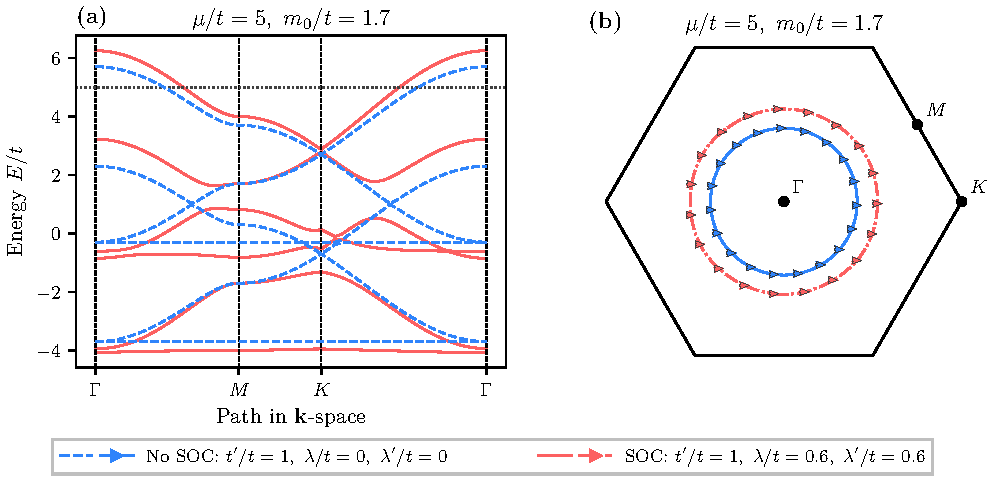
\includegraphics[
        width=\linewidth
    ]{Appendix/homogenous/homogenous_nonbreathing.pdf}
    \caption{\textbf{Results obtained using the tight-binding Hamiltonian \eqref{eq: bloch-Hamiltonian} for the homogeneous magnetic texture, as depicted in Fig. \ref{fig: magnetic texture homogenous} in the nonbreathing limit without and with SOC, respectively.} (a) Band structure along the high-symmetry path $\Gamma$-$K$-$M$, (b) the in-plane Fermi surface spin textures for the chemical potential $\mu$.}
    \label{fig:homogenous-nonbreathing}
\end{figure}

Finally, Fig.~\ref{fig:homogenous-notexture} compares the band structures (a),(b) without a magnetic texture with those for the (c),(d) homogeneous texture. 
For $t'= \lambda = \lambda'=0$, the nonmagnetic kagome lattice has two distinct flat bands, with one of them being orbital degenerate. The flatness stems from the fact that the electrons cannot propagate in the lattice because of a missing hopping on the upward-facing triangles. One might expect three flat bands, however, it can easily be verified by solving the Hamiltonian
\begin{align}
    \mathfrak{H}(\mathbf{k}) = t\begin{pmatrix}
        0&   e^{-i\mathbf{k}\cdot \mathbf{a}_1} &   e^{i\mathbf{k}\cdot \mathbf{a}_3} \\
          e^{i\mathbf{k}\cdot \mathbf{a}_1} & 0 &    e^{-i\mathbf{k}\cdot \mathbf{a}_2} \\
        e^{-i\mathbf{k}\cdot \mathbf{a}_3} &   e^{i\mathbf{k}\cdot \mathbf{a}_2} & 0 
    \end{pmatrix},
\end{align}
following from $\hat{t}_i = t \hat{I}_2$ and $\hat{t}' = t'\hat{I}_2 = 0$ and removing the spin dependence due to a spin-independent Hamiltonian. Solving the matrix with the earlier defined cell-connection vectors $\mathbf{a}_i$, which sum to zero, the eigenvalues $E_+ = 2t$ and the twofold degenerate $E_- = -t$ are obtained. Therefore, the upper band is twofold degenerate and the lower one fourfold degenerate, including an orbital degeneracy. 
Now, by adding SOC with $\lambda'=t'=0$, we obtain three flat bands, occurring due to a broken orbital degeneracy. Note that the bands are still Kramers-degenerate. 

\begin{figure}[tbhp]
    \centering
    \begin{subfigure}[t]{0.85\textwidth}
        \centering
        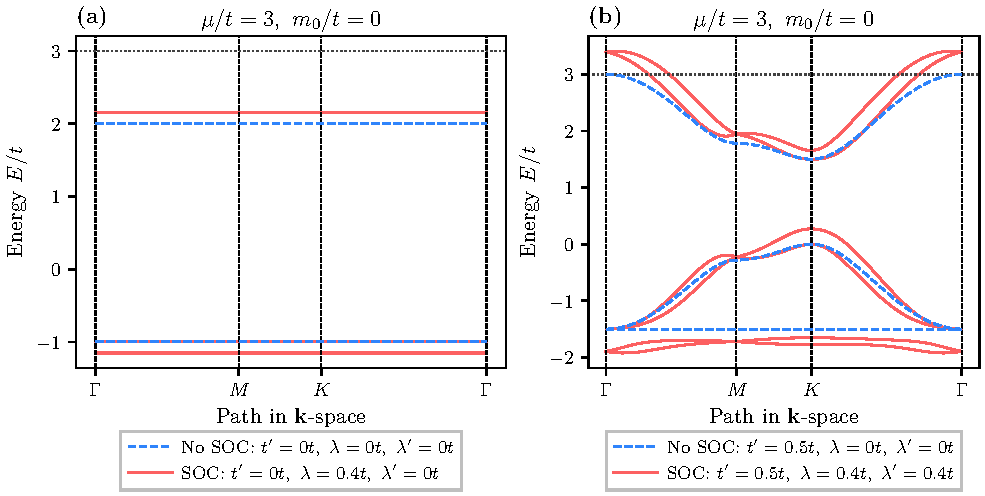
\includegraphics[
            width=\linewidth
        ]{Appendix/no texture vs homogenous/no texture.pdf}
        
    \end{subfigure}
    \vspace{2cm}
    \begin{subfigure}[t]{0.85\textwidth}
        \centering
        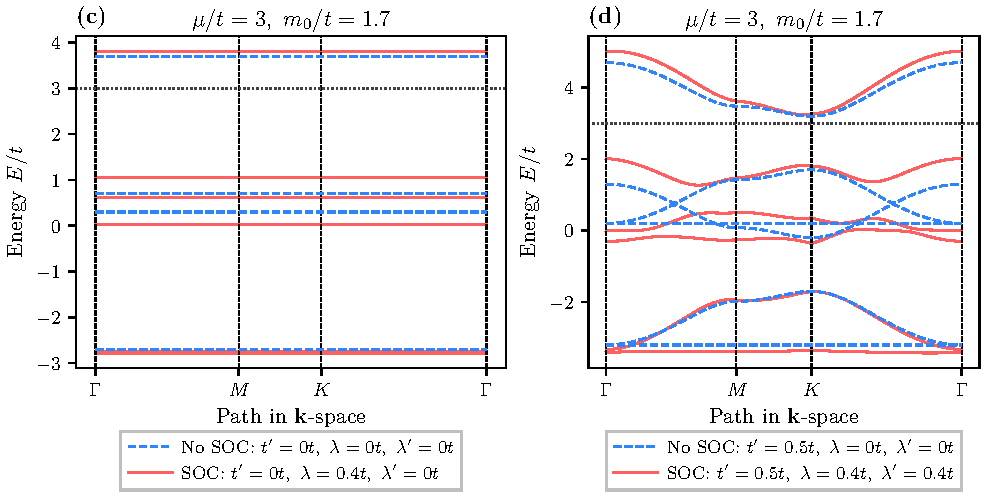
\includegraphics[
            width=\linewidth
        ]{Appendix/no texture vs homogenous/texture.pdf}
        
    \end{subfigure}
    \caption{\textbf{The computed band structure along the high-symmetry path $\Gamma$-$K$-$M$ for the Hamiltonian in Eq.~\eqref{eq: bloch-Hamiltonian}.} Results for no magnetic texture (a) without SOC, (b) with SOC and for an homogeneous magnetic texture, depicted in Fig.~\ref{fig: magnetic texture homogenous}, (c) without SOC and (d) with SOC.}
    \label{fig:homogenous-notexture}
\end{figure}

By adding a magnetic texture, the Kramers degeneracy is broken and therefore there are twice as many distinct bands, due to the magnetic texture breaking time-reversal and the lack of an antiunitary symmetry protecting the degeneracy.

Furthermore, by adding hopping on upward-facing triangles, so $t'\neq0$ or $\lambda'\neq 0$, dispersive bands are obtained, as seen in Fig.~\ref{fig:homogenous-notexture} (b), (d). For no SOC and no magnetic texture, Kramers pairs are expected, resulting in three twofold degenerate bands, as observed.  These bands are split by adding SOC or a magnetic texture, therefore resulting in six dispersive bands.
In the absence of SOC for a breathing lattice, it is interesting to note that there still exists a twofold degenerate flat band for no magnetic texture, or a flat band for the magnetic lattice. This arises from the lattice and magnetic geometry, leading to destructive interference. A detailed analysis of this flat band is beyond the scope of this work.
None of the not-treated cases, for example breathing lattice with SOC, are not analyzed in detail because we expect up to six dispersive bands in all of them, where degeneracies, forced by the lattice and magnetic geometry may occur. 







\thispagestyle{empty}
~

\thispagestyle{empty}
\printbibliography

\newpage


\chapter*{Acknowledgments}
First and foremost, I would like to thank Prof. Dr. Mathias S. Scheurer for giving me the opportunity and freedom to work on this project at the ITP III. Also, I want to thank Dr. Jessica Almeida for always being available for questions of any kind and Dr. Nicolai Lang for all the technical support.\\
I also want to give a huge thank you to my mother, father, and Hanna, who always gave me encouragement and support throughout this time.
Lastly, I would like to thank my office colleagues, all members of the institute and friends, especially Kevin, who made every bit of free time I had very enjoyable. 


\end{document}